
%% bare_jrnl.tex
%% V1.4
%% 2012/12/27
%% by Michael Shell
%% see http://www.michaelshell.org/
%% for current contact information.
%%
%% This is a skeleton file demonstrating the use of IEEEtran.cls
%% (requires IEEEtran.cls version 1.8 or later) with an IEEE journal paper.
%%
%% Support sites:
%% http://www.michaelshell.org/tex/ieeetran/
%% http://www.ctan.org/tex-archive/macros/latex/contrib/IEEEtran/
%% and
%% http://www.ieee.org/



% *** Authors should verify (and, if needed, correct) their LaTeX system  ***
% *** with the testflow diagnostic prior to trusting their LaTeX platform ***
% *** with production work. IEEE's font choices can trigger bugs that do  ***
% *** not appear when using other class files.                            ***
% The testflow support page is at:
% http://www.michaelshell.org/tex/testflow/


%%*************************************************************************
%% Legal Notice:
%% This code is offered as-is without any warranty either expressed or
%% implied; without even the implied warranty of MERCHANTABILITY or
%% FITNESS FOR A PARTICULAR PURPOSE! 
%% User assumes all risk.
%% In no event shall IEEE or any contributor to this code be liable for
%% any damages or losses, including, but not limited to, incidental,
%% consequential, or any other damages, resulting from the use or misuse
%% of any information contained here.
%%
%% All comments are the opinions of their respective authors and are not
%% necessarily endorsed by the IEEE.
%%
%% This work is distributed under the LaTeX Project Public License (LPPL)
%% ( http://www.latex-project.org/ ) version 1.3, and may be freely used,
%% distributed and modified. A copy of the LPPL, version 1.3, is included
%% in the base LaTeX documentation of all distributions of LaTeX released
%% 2003/12/01 or later.
%% Retain all contribution notices and credits.
%% ** Modified files should be clearly indicated as such, including  **
%% ** renaming them and changing author support contact information. **
%%
%% File list of work: IEEEtran.cls, IEEEtran_HOWTO.pdf, bare_adv.tex,
%%                    bare_conf.tex, bare_jrnl.tex, bare_jrnl_compsoc.tex,
%%                    bare_jrnl_transmag.tex
%%*************************************************************************

% Note that the a4paper option is mainly intended so that authors in
% countries using A4 can easily print to A4 and see how their papers will
% look in print - the typesetting of the document will not typically be
% affected with changes in paper size (but the bottom and side margins will).
% Use the testflow package mentioned above to verify correct handling of
% both paper sizes by the user's LaTeX system.
%
% Also note that the "draftcls" or "draftclsnofoot", not "draft", option
% should be used if it is desired that the figures are to be displayed in
% draft mode.
%
\documentclass[journal]{IEEEtran}
%
% If IEEEtran.cls has not been installed into the LaTeX system files,
% manually specify the path to it like:
% \documentclass[journal]{../sty/IEEEtran}

%\linespread{2.5}



% Some very useful LaTeX packages include:
% (uncomment the ones you want to load)


% *** MISC UTILITY PACKAGES ***
%
%\usepackage{ifpdf}
% Heiko Oberdiek's ifpdf.sty is very useful if you need conditional
% compilation based on whether the output is pdf or dvi.
% usage:
% \ifpdf
%   % pdf code
% \else
%   % dvi code
% \fi
% The latest version of ifpdf.sty can be obtained from:
% http://www.ctan.org/tex-archive/macros/latex/contrib/oberdiek/
% Also, note that IEEEtran.cls V1.7 and later provides a builtin
% \ifCLASSINFOpdf conditional that works the same way.
% When switching from latex to pdflatex and vice-versa, the compiler may
% have to be run twice to clear warning/error messages.






% *** CITATION PACKAGES ***
%
%\usepackage{cite}
% cite.sty was written by Donald Arseneau
% V1.6 and later of IEEEtran pre-defines the format of the cite.sty package
% \cite{} output to follow that of IEEE. Loading the cite package will
% result in citation numbers being automatically sorted and properly
% "compressed/ranged". e.g., [1], [9], [2], [7], [5], [6] without using
% cite.sty will become [1], [2], [5]--[7], [9] using cite.sty. cite.sty's
% \cite will automatically add leading space, if needed. Use cite.sty's
% noadjust option (cite.sty V3.8 and later) if you want to turn this off
% such as if a citation ever needs to be enclosed in parenthesis.
% cite.sty is already installed on most LaTeX systems. Be sure and use
% version 4.0 (2003-05-27) and later if using hyperref.sty. cite.sty does
% not currently provide for hyperlinked citations.
% The latest version can be obtained at:
% http://www.ctan.org/tex-archive/macros/latex/contrib/cite/
% The documentation is contained in the cite.sty file itself.






% *** GRAPHICS RELATED PACKAGES ***
%
\ifCLASSINFOpdf
  % \usepackage[pdftex]{graphicx}
  % declare the path(s) where your graphic files are
  % \graphicspath{{../pdf/}{../jpeg/}}
  % and their extensions so you won't have to specify these with
  % every instance of \includegraphics
  % \DeclareGraphicsExtensions{.pdf,.jpeg,.png}
\else
  % or other class option (dvipsone, dvipdf, if not using dvips). graphicx
  % will default to the driver specified in the system graphics.cfg if no
  % driver is specified.
  % \usepackage[dvips]{graphicx}
  % declare the path(s) where your graphic files are
  % \graphicspath{{../eps/}}
  % and their extensions so you won't have to specify these with
  % every instance of \includegraphics
  % \DeclareGraphicsExtensions{.eps}
\fi
% graphicx was written by David Carlisle and Sebastian Rahtz. It is
% required if you want graphics, photos, etc. graphicx.sty is already
% installed on most LaTeX systems. The latest version and documentation
% can be obtained at: 
% http://www.ctan.org/tex-archive/macros/latex/required/graphics/
% Another good source of documentation is "Using Imported Graphics in
% LaTeX2e" by Keith Reckdahl which can be found at:
% http://www.ctan.org/tex-archive/info/epslatex/
%
% latex, and pdflatex in dvi mode, support graphics in encapsulated
% postscript (.eps) format. pdflatex in pdf mode supports graphics
% in .pdf, .jpeg, .png and .mps (metapost) formats. Users should ensure
% that all non-photo figures use a vector format (.eps, .pdf, .mps) and
% not a bitmapped formats (.jpeg, .png). IEEE frowns on bitmapped formats
% which can result in "jaggedy"/blurry rendering of lines and letters as
% well as large increases in file sizes.
%
% You can find documentation about the pdfTeX application at:
% http://www.tug.org/applications/pdftex





% *** MATH PACKAGES ***
%
%\usepackage[cmex10]{amsmath}
% A popular package from the American Mathematical Society that provides
% many useful and powerful commands for dealing with mathematics. If using
% it, be sure to load this package with the cmex10 option to ensure that
% only type 1 fonts will utilized at all point sizes. Without this option,
% it is possible that some math symbols, particularly those within
% footnotes, will be rendered in bitmap form which will result in a
% document that can not be IEEE Xplore compliant!
%
% Also, note that the amsmath package sets \interdisplaylinepenalty to 10000
% thus preventing page breaks from occurring within multiline equations. Use:
%\interdisplaylinepenalty=2500
% after loading amsmath to restore such page breaks as IEEEtran.cls normally
% does. amsmath.sty is already installed on most LaTeX systems. The latest
% version and documentation can be obtained at:
% http://www.ctan.org/tex-archive/macros/latex/required/amslatex/math/





% *** SPECIALIZED LIST PACKAGES ***
%
%\usepackage{algorithmic}
\usepackage{algpseudocode}
% algorithmic.sty was written by Peter Williams and Rogerio Brito.
% This package provides an algorithmic environment fo describing algorithms.
% You can use the algorithmic environment in-text or within a figure
% environment to provide for a floating algorithm. Do NOT use the algorithm
% floating environment provided by algorithm.sty (by the same authors) or
% algorithm2e.sty (by Christophe Fiorio) as IEEE does not use dedicated
% algorithm float types and packages that provide these will not provide
% correct IEEE style captions. The latest version and documentation of
% algorithmic.sty can be obtained at:
% http://www.ctan.org/tex-archive/macros/latex/contrib/algorithms/
% There is also a support site at:
% http://algorithms.berlios.de/index.html
% Also of interest may be the (relatively newer and more customizable)
% algorithmicx.sty package by Szasz Janos:
% http://www.ctan.org/tex-archive/macros/latex/contrib/algorithmicx/




% *** ALIGNMENT PACKAGES ***
%
%\usepackage{array}
% Frank Mittelbach's and David Carlisle's array.sty patches and improves
% the standard LaTeX2e array and tabular environments to provide better
% appearance and additional user controls. As the default LaTeX2e table
% generation code is lacking to the point of almost being broken with
% respect to the quality of the end results, all users are strongly
% advised to use an enhanced (at the very least that provided by array.sty)
% set of table tools. array.sty is already installed on most systems. The
% latest version and documentation can be obtained at:
% http://www.ctan.org/tex-archive/macros/latex/required/tools/


% IEEEtran contains the IEEEeqnarray family of commands that can be used to
% generate multiline equations as well as matrices, tables, etc., of high
% quality.




% *** SUBFIGURE PACKAGES ***
%\ifCLASSOPTIONcompsoc
%  \usepackage[caption=false,font=normalsize,labelfont=sf,textfont=sf]{subfig}
%\else
%  \usepackage[caption=false,font=footnotesize]{subfig}
%\fi
% subfig.sty, written by Steven Douglas Cochran, is the modern replacement
% for subfigure.sty, the latter of which is no longer maintained and is
% incompatible with some LaTeX packages including fixltx2e. However,
% subfig.sty requires and automatically loads Axel Sommerfeldt's caption.sty
% which will override IEEEtran.cls' handling of captions and this will result
% in non-IEEE style figure/table captions. To prevent this problem, be sure
% and invoke subfig.sty's "caption=false" package option (available since
% subfig.sty version 1.3, 2005/06/28) as this is will preserve IEEEtran.cls
% handling of captions.
% Note that the Computer Society format requires a larger sans serif font
% than the serif footnote size font used in traditional IEEE formatting
% and thus the need to invoke different subfig.sty package options depending
% on whether compsoc mode has been enabled.
%
% The latest version and documentation of subfig.sty can be obtained at:
% http://www.ctan.org/tex-archive/macros/latex/contrib/subfig/




% *** FLOAT PACKAGES ***
%
%\usepackage{fixltx2e}
% fixltx2e, the successor to the earlier fix2col.sty, was written by
% Frank Mittelbach and David Carlisle. This package corrects a few problems
% in the LaTeX2e kernel, the most notable of which is that in current
% LaTeX2e releases, the ordering of single and double column floats is not
% guaranteed to be preserved. Thus, an unpatched LaTeX2e can allow a
% single column figure to be placed prior to an earlier double column
% figure. The latest version and documentation can be found at:
% http://www.ctan.org/tex-archive/macros/latex/base/


%\usepackage{stfloats}
% stfloats.sty was written by Sigitas Tolusis. This package gives LaTeX2e
% the ability to do double column floats at the bottom of the page as well
% as the top. (e.g., "\begin{figure*}[!b]" is not normally possible in
% LaTeX2e). It also provides a command:
%\fnbelowfloat
% to enable the placement of footnotes below bottom floats (the standard
% LaTeX2e kernel puts them above bottom floats). This is an invasive package
% which rewrites many portions of the LaTeX2e float routines. It may not work
% with other packages that modify the LaTeX2e float routines. The latest
% version and documentation can be obtained at:
% http://www.ctan.org/tex-archive/macros/latex/contrib/sttools/
% Do not use the stfloats baselinefloat ability as IEEE does not allow
% \baselineskip to stretch. Authors submitting work to the IEEE should note
% that IEEE rarely uses double column equations and that authors should try
% to avoid such use. Do not be tempted to use the cuted.sty or midfloat.sty
% packages (also by Sigitas Tolusis) as IEEE does not format its papers in
% such ways.
% Do not attempt to use stfloats with fixltx2e as they are incompatible.
% Instead, use Morten Hogholm'a dblfloatfix which combines the features
% of both fixltx2e and stfloats:
%
% \usepackage{dblfloatfix}
% The latest version can be found at:
% http://www.ctan.org/tex-archive/macros/latex/contrib/dblfloatfix/




%\ifCLASSOPTIONcaptionsoff
%  \usepackage[nomarkers]{endfloat}
% \let\MYoriglatexcaption\caption
% \renewcommand{\caption}[2][\relax]{\MYoriglatexcaption[#2]{#2}}
%\fi
% endfloat.sty was written by James Darrell McCauley, Jeff Goldberg and 
% Axel Sommerfeldt. This package may be useful when used in conjunction with 
% IEEEtran.cls'  captionsoff option. Some IEEE journals/societies require that
% submissions have lists of figures/tables at the end of the paper and that
% figures/tables without any captions are placed on a page by themselves at
% the end of the document. If needed, the draftcls IEEEtran class option or
% \CLASSINPUTbaselinestretch interface can be used to increase the line
% spacing as well. Be sure and use the nomarkers option of endfloat to
% prevent endfloat from "marking" where the figures would have been placed
% in the text. The two hack lines of code above are a slight modification of
% that suggested by in the endfloat docs (section 8.4.1) to ensure that
% the full captions always appear in the list of figures/tables - even if
% the user used the short optional argument of \caption[]{}.
% IEEE papers do not typically make use of \caption[]'s optional argument,
% so this should not be an issue. A similar trick can be used to disable
% captions of packages such as subfig.sty that lack options to turn off
% the subcaptions:
% For subfig.sty:
% \let\MYorigsubfloat\subfloat
% \renewcommand{\subfloat}[2][\relax]{\MYorigsubfloat[]{#2}}
% However, the above trick will not work if both optional arguments of
% the \subfloat command are used. Furthermore, there needs to be a
% description of each subfigure *somewhere* and endfloat does not add
% subfigure captions to its list of figures. Thus, the best approach is to
% avoid the use of subfigure captions (many IEEE journals avoid them anyway)
% and instead reference/explain all the subfigures within the main caption.
% The latest version of endfloat.sty and its documentation can obtained at:
% http://www.ctan.org/tex-archive/macros/latex/contrib/endfloat/
%
% The IEEEtran \ifCLASSOPTIONcaptionsoff conditional can also be used
% later in the document, say, to conditionally put the References on a 
% page by themselves.




% *** PDF, URL AND HYPERLINK PACKAGES ***
%
%\usepackage{url}
% url.sty was written by Donald Arseneau. It provides better support for
% handling and breaking URLs. url.sty is already installed on most LaTeX
% systems. The latest version and documentation can be obtained at:
% http://www.ctan.org/tex-archive/macros/latex/contrib/url/
% Basically, \url{my_url_here}.




% *** Do not adjust lengths that control margins, column widths, etc. ***
% *** Do not use packages that alter fonts (such as pslatex).         ***
% There should be no need to do such things with IEEEtran.cls V1.6 and later.
% (Unless specifically asked to do so by the journal or conference you plan
% to submit to, of course. )


% correct bad hyphenation here
%\hyphenation{op-tical net-works semi-conduc-tor}

\usepackage{verbatim}
\usepackage{color, colortbl}
\definecolor{Gray}{gray}{0.9}
\usepackage{graphicx}
\usepackage{rotating}
\usepackage{multirow}
\usepackage{url}

\newcommand{\graphicthird}[1]
{\includegraphics[width=.27\textwidth,height=.27\textheight,keepaspectratio]{#1}}

\newcommand{\thirdlabel}[1]
{\multicolumn{1}{|c|}{\raisebox{.15\textwidth}{\rotatebox[origin=c]{90}{\textbf{\em #1}}}}}

\begin{document}
%
% paper title
% can use linebreaks \\ within to get better formatting as desired
% Do not put math or special symbols in the title.
\title{Analysis of Cartesian Genetic Programming's Evolutionary Mechanisms}
%
%
% author names and IEEE memberships
% note positions of commas and nonbreaking spaces ( ~ ) LaTeX will not break
% a structure at a ~ so this keeps an author's name from being broken across
% two lines.
% use \thanks{} to gain access to the first footnote area
% a separate \thanks must be used for each paragraph as LaTeX2e's \thanks
% was not built to handle multiple paragraphs
%

%\author{Michael~Shell,~\IEEEmembership{Member,~IEEE,}
%        John~Doe,~\IEEEmembership{Fellow,~OSA,}
%        and~Jane~Doe,~\IEEEmembership{Life~Fellow,~IEEE}% <-this % stops a space
\author{Brian~W.~Goldman, William~F.~Punch}
%\thanks{M. Shell is with the Department
%of Electrical and Computer Engineering, Georgia Institute of Technology, Atlanta,
%GA, 30332 USA e-mail: (see http://www.michaelshell.org/contact.html).}% <-this % stops a space
%\thanks{J. Doe and J. Doe are with Anonymous University.}% <-this % stops a space
%\thanks{Manuscript received April 19, 2005; revised December 27, 2012.}}

% note the % following the last \IEEEmembership and also \thanks - 
% these prevent an unwanted space from occurring between the last author name
% and the end of the author line. i.e., if you had this:
% 
% \author{....lastname \thanks{...} \thanks{...} }
%                     ^------------^------------^----Do not want these spaces!
%
% a space would be appended to the last name and could cause every name on that
% line to be shifted left slightly. This is one of those "LaTeX things". For
% instance, "\textbf{A} \textbf{B}" will typeset as "A B" not "AB". To get
% "AB" then you have to do: "\textbf{A}\textbf{B}"
% \thanks is no different in this regard, so shield the last } of each \thanks
% that ends a line with a % and do not let a space in before the next \thanks.
% Spaces after \IEEEmembership other than the last one are OK (and needed) as
% you are supposed to have spaces between the names. For what it is worth,
% this is a minor point as most people would not even notice if the said evil
% space somehow managed to creep in.



% The paper headers
\markboth{IEEE Transactions on Evolutionary Computation,~Vol.~\#\#, No.~\#, Month~Year}%
{IEEE Transactions on Evolutionary Computation,~Vol.~\#\#, No.~\#, Month~Year}
% The only time the second header will appear is for the odd numbered pages
% after the title page when using the twoside option.
% 
% *** Note that you probably will NOT want to include the author's ***
% *** name in the headers of peer review papers.                   ***
% You can use \ifCLASSOPTIONpeerreview for conditional compilation here if
% you desire.




% If you want to put a publisher's ID mark on the page you can do it like
% this:
%\IEEEpubid{0000--0000/00\$00.00~\copyright~2012 IEEE}
% Remember, if you use this you must call \IEEEpubidadjcol in the second
% column for its text to clear the IEEEpubid mark.



% use for special paper notices
%\IEEEspecialpapernotice{(Invited Paper)}

% make the title area
\maketitle

% As a general rule, do not put math, special symbols or citations
% in the abstract or keywords.
\begin{abstract}
Understanding how search operators interact with solution representation is
a critical step to improving search.
In Cartesian Genetic Programming (CGP), and Genetic Programming (GP)
in general, the complex genotype to phenotype map makes achieving this understanding a
challenge.  By examining aspects such as tuned parameter values, the search quality of CGP variants at different
problem difficulties, node behavior, and offspring replacement properties we
seek to better understand the characteristics of CGP search.  Our focus is twofold:
creating methods to prevent wasted CGP evaluations (\emph{Skip}, \emph{Accumulate},
and \emph{Single}) and creating methods to overcome CGP's search limitations imposed by
genome ordering (\emph{Reorder} and \emph{DAG}).

Our results show that most CGP techniques evolve genomes that
are highly inactive, very redundant, and full of seemingly useless constants.
On some tested problems we found less than 1\% of the genome was actually required to
encode the evolved solution.
Furthermore, traditional CGP ordering results in large portions of the genome
that are never used by any ancestor of the evolved solution.
\emph{Reorder} and \emph{DAG} allow evolution to utilize the entire genome.
More generally, our
results suggest that \emph{Skip-Reorder} and \emph{Single-Reorder}
are most likely to solve hard problems using the least number of evaluations and
the least amount of time while better avoiding degenerate
behavior.

\end{abstract}

% Note that keywords are not normally used for peerreview papers.
\begin{IEEEkeywords}
Cartesian genetic programming (CGP), Analysis
\end{IEEEkeywords}






% For peer review papers, you can put extra information on the cover
% page as needed:
% \ifCLASSOPTIONpeerreview
% \begin{center} \bfseries EDICS Category: 3-BBND \end{center}
% \fi
%
% For peerreview papers, this IEEEtran command inserts a page break and
% creates the second title. It will be ignored for other modes.
\IEEEpeerreviewmaketitle



\section{Introduction}
% The very first letter is a 2 line initial drop letter followed
% by the rest of the first word in caps.
% 
% form to use if the first word consists of a single letter:
% \IEEEPARstart{A}{demo} file is ....
% 
% form to use if you need the single drop letter followed by
% normal text (unknown if ever used by IEEE):
% \IEEEPARstart{A}{}demo file is ....
% 
% Some journals put the first two words in caps:
% \IEEEPARstart{T}{his demo} file is ....
% 
% Here we have the typical use of a "T" for an initial drop letter
% and "HIS" in caps to complete the first word.
\IEEEPARstart{W}{hile effective} evolutionary methods are often simple to design
and implement, discerning the reason that system
leads to effective search can be challenging.
This is exceptionally
true for Genetic Programming (GP), which often employs both nontrivial
genotype to phenotype maps and operators that act on genotypes without regard to
phenotypic impact.  Yet understanding the root causes of evolutionary success
and failure is critical to improving existing techniques, designing new techniques,
and understanding how and where to apply each optimization system.

There have been a number of previous studies into various aspects of GP evolution.
For instance~\cite{daida3:2003:treebias} showed how a tree's shape effects its evolvability
regardless of phenotype,
resulting in the use of new grammar based operations~\cite{xuan:2006:grammar}.
Analysis of the root cause of bloat has helped to inform methods for controlling
bloat~\cite{luke:2006:bloat}.

In this work we set out to develop a deeper understanding of what makes Cartesian
Genetic Programming (CGP) an effective evolutionary optimizer.
Previous studies of CGP's evolutionary mechanisms have
focused on bloat~\cite{miller:2001:bloat},
neutrality~\cite{vassilev:2000:neutrality}, and structural bias~\cite{payne:2009:bias}.
We shall focus on the interaction between mutation and genome ordering.
%NEW
While these features of CGP have trivial definitions, we will argue, using
experimentation and analysis of alternatives, that they have a great deal
of impact on search success.
%/NEW

\begin{comment}
In Section~\ref{sec:cgp} we provide
an introduction to CGP, with sufficient background to put later sections into
context.  Section~\ref{sec:duplicate} describes previous work on preventing mutation
from creating identifiably wasted evaluations.
Section~\ref{sec:ordering} discusses the impact of CGP's genome ordering,
along with methods to both examine and bypass the limitations imposed by that ordering.
Each technique is then rigorously tuned and qualitatively compared on a collection
of benchmarks in Section~\ref{sec:quality}.  Section~\ref{sec:analysis} then
provides a deep look into the details of CGP's search, and how each method impacts
search, with final remarks given in Section~\ref{sec:conclusion}.
\end{comment}

\section{Cartesian Genetic Programming}
\label{sec:cgp}
Cartesian Genetic Programming (CGP) was originally proposed as a method for general
genetic programming in~\cite{miller:2000:CGPorigin}.  While its name comes from
its original application evolving circuits on a two dimensional grid, modern CGP can
represent any directed acyclic graph (DAG), and has been utilized in applications such as binary
circuits~\cite{walker:2008:cgpmodules},
robot controllers~\cite{harding:2005:robots},
neural networks~\cite{khan:2010:cgpann},
image classifiers~\cite{harding:2012:mtcgp},
and regression~\cite{harding:2009:smcgp}.

CGP represents DAGs using a linear genome of integer values.  Each node in the
DAG is encoded as a tuple of genes, with one gene specifying the function
the node applies to its inputs, and the remaining genes expressing where the
node takes input from.  Nodes can take input from either a problem input or
any node preceding them in the linear genome.  Restricting connections in this way
prevents the creation of cycles, while still allowing CGP to reuse values.  This is
in contrast to tree based GP, which must duplicate functionality everywhere the same value is needed.
To complete the representation, a set
of extra genes are included at the end of the genome to specify which nodes or
input locations to use as function outputs.

As both output locations and information flow in the DAG are evolvable, often
only a tiny fraction of the genome participates in creating the
output values.  These nodes are referred to as ``active,'' with the nodes not
being used to create output values referred to as ``inactive.''  Inactive nodes
allow CGP individuals to drift genetically, as they can be mutated without effecting
the fitness of the individual.  This genetic drift can then be incorporated, as
mutation can change the DAG structure causing previously inactive nodes to become
active.  Previous work suggests CGP is most efficient when up to 95\% of the genome
is inactive~\cite{miller:2006:redundancy}, while more recent work suggests this may
be a result of hidden parsimony pressure in CGP~\cite{goldman:2013:ordering}.

CGP uses very simple evolutionary mechanisms.  The most common evolutionary strategy
is $\mu + \lambda$ where $\mu \leftarrow 1$ and $\lambda \leftarrow 4$.
This means during each generation a single parent produces four offspring using
mutation.  The best offspring then competes with the parent,\footnote{Ties are broken
randomly.} with the offspring
replacing the parent if it is no less fit.  This replacement strategy encourages
neutral drift.
%NEW
In CGP mutation is done in a myriad of nearly synonymous ways.  Here we mutate
%/NEW
each gene of each node at a set probability, where mutation
involves changing a gene randomly to some different valid value.  For example,
if a function gene is chosen for mutation, its new value is randomly chosen from
all possible functions, excluding the gene's current value.
%NEW
This version of mutation was chosen to allow precise prediction of changes
in gene value necessarily in later sections.
%/NEW
Combined,
this form of CGP can be viewed as a stochastic hill climber with neutrality.
For a more in depth description of CGP, see~\cite{miller:2011:chapter2}.

\section{Duplicate Evaluation Avoidance}
\label{sec:duplicate}
CGP's mutation operator is traditionally applied to both active and inactive genes uniformly.
This has the
potential to create offspring who's only mutated genes are in inactive nodes.
These offspring are actively identical (contain identical active genes) to their
parents, and therefore by definition have identical fitness to their parents.
As such, re-evaluating these individuals is computationally wasteful as their fitness
is known.
Detecting duplicated individuals can be done without significant overhead since
finding the set of active nodes is already done prior to
evaluation~\cite{vasicek:2012:efficient}.
Our previous work~\cite{goldman:2013:cgpwaste} has taken an initial look at the
effect this waste can have, and proposed \emph{Skip}, \emph{Accumulate}, and
\emph{Single} as methods for avoiding or preventing these duplicate evaluations.

\begin{comment}
The number of wasted evaluations is
directly related to the mutation probability and the number of active genes.  With
sufficiently high probabilities and enough active genes, the chance of
creating an offspring which is actively identical to its parent is very low.
Yet such a configuration may make it difficult for CGP to optimize, as mutation
is likely to change many active genes in each application.  As was discussed
in~\cite{goldman:2013:cgpwaste}, this can make normal CGP very sensitive to the
mutation probability.
\end{comment}

\subsection{Skip}
The \emph{Skip} method for avoiding duplicate evaluations involves the least
amount of modification from CGP's normal behavior.  After an offspring is produced
and its set of active nodes is determined but before it is evaluated, it is compared
with its parent.  Each gene in each active node is compared for equivalence with
the corresponding gene in the offspring's parent.  If all active genes are found to be equal
then the offspring is not evaluated and is instead given the same fitness
as its parent.
Note that since inactive genes are not compared for equivalence it is still possible
for offspring to genetically differ from their parents.

Because \emph{Skip} does not modify any evolutionary mechanisms found in traditional CGP,
it will produce identical individuals, with a potential reduction in evaluations.
If the mutation probability is high enough relative
to the number of active genes, \emph{Skip} will require the same number of evaluations as traditional CGP, since
the probability of an offspring being actively identical to its parent is effectively zero.
When the mutation probability is low enough relative to the number of active genes, some number of
offspring will be actively identical to their parents, resulting in a reduction in evaluations
but no change in the evolutionary trajectory.

%NEW
This technique incurs a minor increase in runtime, as each active gene in the
offspring must be compared against the parent's gene at the same locus.
This operation is at most linear in genome size.  Yet
on problems where evaluation is even somewhat expensive, the evaluations prevented
by performing this check will result in a net reduction in runtime.
%/NEW

We would expect both intuitively and from our initial
experimentation~\cite{goldman:2013:cgpwaste} that \emph{Skip} will be less sensitive
to the mutation probability than normal CGP.  We would also expect \emph{Skip} to use a lower
mutation probability than normal CGP when both are optimized to reduce evaluations.
The former comes from the fact that in normal CGP any mutation probability that has a significant
chance of creating offspring actively identical to their parents wastes
evaluations.  In \emph{Skip} there are only two penalties for reducing the
mutation probability.  From an evolutionary standpoint, if search becomes trapped in a local optima, low mutation
probabilities may have increased difficulty escaping to find the global optimum.  From a performance standpoint,
exceptionally low mutation probabilities may spend a prohibitive amount of time
attempting to produce an evaluable offspring.
Note that these penalties also exist in normal CGP.

\subsection{Accumulate}
Similar to \emph{Skip}, \emph{Accumulate} works by adding a step between offspring
creation and offspring evaluation.  Instead of skipping evaluations when offspring
are determined to be actively identical to their parents, \emph{Accumulate} enters
into a cycle of repeated mutation until an individual worth evaluating is created.
To understand this technique, consider an example where the parent $P$ produces
the offspring $F_0$ using mutation. If $F_0$ is actively identical to $P$, $F_0$
creates its own offspring $F_1$ using mutation.  This process of $F_i$ producing
$F_{i+1}$ continues until $F_n$ is produced, where $F_n$ is not actively identical
to $P$.  $F_n$ is then evaluated.  If $F_n$ is no worse than $P$, it replaces
$F_0$, and evolution continues as though $P$ had produced $F_n$ directly.  If
$F_n$ is worse than $P$, $F_{n-1}$ replaces $F_0$, as $F_{n-1}$ has accumulated
the most mutations to inactive genes without reducing fitness.  Note that
the mutation used each time is identical to normal CGP's mutation, such that
$F_n$ will have one or more active genes different from $P$.  Furthermore, even
though this technique produces $n+1$ individuals, only $F_n$ is evaluated.
Viewed in another way, \emph{Accumulate} performs a micro evolution on each offspring
before it is evaluated, with an emphasis on encouraging neutral drift.

Previous experimentation has shown that \emph{Accumulate} acts very similarly to
\emph{Skip}~\cite{goldman:2013:cgpwaste}, with the exception that \emph{Accumulate}
favors lower mutation probabilities when tuned to reduce evaluations to success. While at first these algorithms may appear
quite different, further consideration shows how they are similar.  In \emph{Skip}
any actively identical offspring that is produced is likely to be selected as we expect mutations to
active genes to more often reduce fitness than improve it.  In the next generation
this actively identical offspring is then mutated again, with its lineage likely
continuing until it finally does mutate one or more active genes.  At this point, if the
mutant is better it replaces the parent, otherwise the parent, which has been accumulating
mutations to inactive genes, is kept.  In this way \emph{Skip} mirrors \emph{Accumulate},
except \emph{Skip} acts over multiple generations instead of compressed into a single generation.

%NEW
Similar to \emph{Skip}, \emph{Accumulate} incurs a minor computation cost in
order to prevent wasting evaluations.  Generating each $F_i$ requires at most
$O(AN)$, where $A$ is the arity of the nodes and $N$ is the number of nodes.
While \emph{Accumulate} may produce many $F_i$ in the process of creating
a single offspring, conceptually \emph{Skip} using the same mutation rate
will create a similar number of total individuals when performing the same
number of evaluations.  As such, we suggest \emph{Accumulate}
will take no more than a constant factor more runtime to produce the same number
of evaluable individuals as \emph{Skip}.  As before, this increase is likely
eclipsed when solving problems with sufficiently time consuming evaluation functions.
%/NEW


\subsection{Single}
While \emph{Skip} and \emph{Accumulate} save evaluations by not evaluating offspring
which are actively identical to their parents, \emph{Single} changes
mutation to ensure that only evaluable offspring are created.  Instead
of mutating each gene at a set probability, \emph{Single} mutates genes at
random until exactly one active gene is mutated.

This modification gives \emph{Single} three properties distinct from the other
forms of duplicate avoidance.  First, \emph{Single} forces offspring to have
an active gene which differs from their parent.  This limits drift as the
mutated active gene must either be to an intron or represent another way to
code a solution of equal quality.  Second, as a benefit of forced changes,
\emph{Single} avoids the overhead of repeatedly generating individuals without
creating an evaluable offspring.  Third, \emph{Single} does not require a mutation
parameter, effectively setting the mutation probability to $\frac{1}{a}$ for active
genes and $\frac{1}{a+1}$ for inactive genes, where $a$ is the number of active genes.

In encodings without inactive genes, limiting mutation to changing exactly one gene
could prevent an algorithm from escaping some types of local optima.  Yet because
CGP allows for inactive genes, \emph{Single} is still able to escape most local
optima using sufficient drift of inactive genes.  When a high percentage of
the genome becomes active or when \emph{Single} is otherwise limited in its ability
to drift due to lack of introns, it does have an increased potential to become stuck.
As will be discussed in Section~\ref{sec:ordering} and was shown in~\cite{goldman:2013:ordering}
this problem of highly active genomes is very unlikely.

%NEW
Conceptually this method could be extended to mutate some number of active genes
before terminating.  Doing so would reintroduce a parameter to govern how many
active genes to mutate.  Our choice of a single mutation allows for the minimal
amount of change to ensure the individual should be evaluated, while mutations
made to inactive genes still give CGP sufficient power in each mutation to escape
local optimums.
%/NEW

\section{Genome Ordering}
\label{sec:ordering}
As was discussed in Section~\ref{sec:cgp}, CGP uses node ordering in the genome
to prevent cycles, by ensuring nodes only receive input from sources that
precede them in the genome.  This restriction does not limit CGP's ability
to represent DAGs, as all DAGs can be serialized to fit this requirement.
However, this representation is likely having an impact on CGP's ability to evolve specific
DAGs~\cite{goldman:2013:ordering}.

Primarily, enforcing node ordering adds artificial limitations to CGP's ability to
connect nodes.  Nodes which can be connected without creating a cycle may
still be prevented from forming that connection because of random genome ordering.
Similarly, it is impossible for adjacent nodes
to ever be connected through an intermediate node.  As a result, useful structures
in the genome may need to be evolved repeatedly in order to find the best
location for that structure in the genome.

Ordering, when combined with the mutation's uniform resetting of connection genes, may be the cause of CGP's
immensely inactive genomes.  As was rigorously defined in our work~\cite{goldman:2013:ordering},
the number of active genes in a genome is expected to scale logarithmically
with genome size, independent of problem application.  Furthermore, the less
active a genome, the lower the likelihood of structure ordering preventing structure
connection.

As an extension to the theory presented in~\cite{goldman:2013:ordering}, we have
derived the formula which predicts the probability a node is active based on its
index, given in Equation~\ref{eq:prob}.
\begin{equation}
p(i) \leftarrow 1 - (\frac{N+I-1}{N+I})^O \cdot \prod_{j=i+1}^{N} 1 - p(j) \cdot (1-(\frac{j+I-1}{j+I})^A)
\label{eq:prob}
\end{equation}
In this equation, $i$ is the index of the working node, $N$ is the genome size, $I$ is the number of input locations,
$O$ is the number of output locations, and $A$ is the arity of each node.
This equation is constructed as a negation, such that we determine the probability
the node is not active due to each potential source that could make it active.
The product term calculates the probability that the node at index $j$ is connected to the
node at index $i$, multiplied by the probability that the node at index $j$ is active.  This is
negated to determine the probability node $i$ is not active because of node $j$.
All together, the product term calculates the probability that no active node is
connected to the node at index $i$.  Nodes can also become active if they are directly
connected to by an output location.  As such the product is scaled by the probability
that all output locations connect to inputs or nodes not at index $i$.  This
formula assumes only operator bias, not selective pressure, is acting on the
genome.

\begin{comment}
\begin{figure}
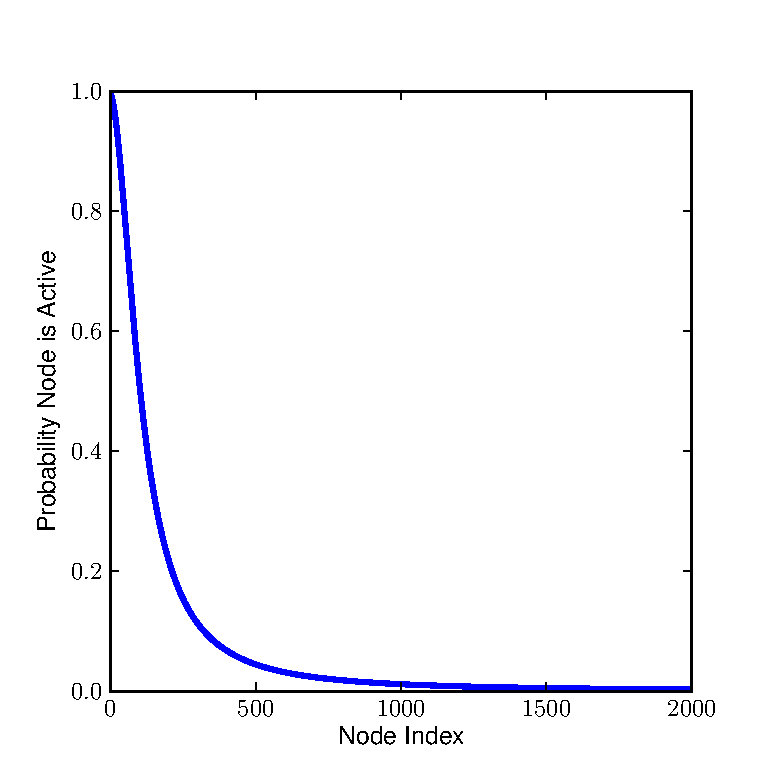
\includegraphics[width=\columnwidth,height=\textheight,keepaspectratio]{active_prob}
\caption{Plot of Equation~\ref{eq:prob} describing the probability that a node
         at a given index will be active.  $N=2000, A=2, I=6, O=6$.
         Predicts approximately 160 total active nodes, with 80\% of the first
         100 nodes active and 4\% of the remaining 1900 nodes active.}
\label{fig:prob}
\end{figure}

From Figure~\ref{fig:prob} it is clear that nodes near the beginning of the genome
are almost certainly going to be active, while nodes in the last three quarters
of the genome are almost never going to be active.
\end{comment}
%NEW
Substituting $N=2000$, $A=2$, $I=6$, $O=6$ into Equation~\ref{eq:prob}
predicts only 160 active nodes, with 80\% of the first 100 nodes expected to be
active while just 4\% of the remaining 1900 nodes are expected to be active.
%/NEW

To rectify these issues and examine CGP without ordering bias, \cite{goldman:2013:ordering}
created \emph{Reorder} and \emph{DAG} as methods for genome ordering.
%NEW
For clarity, we shall refer to CGP's historical ordering method of enforcing
only forward connections as \emph{Normal}.
%/NEW

%NEW
It is important to note that Equation~\ref{eq:prob} does not apply to all variants of CGP.
For instance, the early versions of CGP~\cite{miller:2011:chapter2} which utilize a
levels back parameter $L$ will have
a flat active probability for all nodes at least $L$ nodes from the start and $L$ nodes from the end
of the genome.  Yet this does not remove the issue of artificially limiting connections,
and in fact adds many new limitations.  More recently,~\cite{cai:2005:ircgp} proposed
a method which reassembled the genome using semantic cues, which circumvents the
forward only limitation in \emph{Normal}.
%/NEW
\subsection{Reorder}
\label{sec:reorder}
The \emph{Reorder} method shuffles an existing genome's node ordering without
changing node behavior.  This is possible because for a given node, there can
be a large number of other nodes which have no required ordering,
as they neither take input (directly or indirectly) from the node nor provide their
output (directly or indirectly) to the node.  In general, this process works by assigning nodes new
locations in the genome at random once all of the nodes they take input from have been assigned
locations earlier in the genome.

The first step in performing \emph{Reorder} on a genome is to create
data structures to store direct connection relationships.  These structures are used
to determine in constant time all connections incident on a node, and 
can be built in order $O(AN)$ time, where $A$ is the arity of the nodes
and $N$ is the number of nodes.

With this preprocessing complete, the \Call{RandomSerialization}{} algorithm given in Figure~\ref{fig:reorder}
is used to assign each node a new location in the modified genome.
It starts by constructing the \emph{addable} set, which contains all nodes who's direct
dependencies have already been added.  Initially this contains only the input locations.
Once a node is assigned a location, all of the nodes that depend on its output
have that dependency marked as satisfied.  Once all of a node's dependencies
are satisfied, it can be put into \emph{addable}.  In this way, nodes are
randomly removed from \emph{addable}, assigned the next possible location
in the genome, with new nodes added to \emph{addable} as they becomes semantically
viable.  Iteration ends when all nodes have been assigned new locations.
\Call{RandomSerialization}{} requires $O(AN)$, as there can be only $N$ iterations,
with each iteration updating a distinct subset of the $AN$ dependencies.

\begin{figure}
  \begin{algorithmic}
    \Procedure{RandomSerialization}{}
    \State $addable \leftarrow input\_locations$
    \State $index \leftarrow |input\_locations|$
    \State $new\_loc \leftarrow \emptyset$
    \While{$|addable| > 0$}
      \State $working \leftarrow randpop(addable)$
      \If{$working \notin input\_locations$}
        \State $new\_loc[working] \leftarrow index$
        \State $index \leftarrow index + 1$
      \EndIf
      \ForAll{$link \in feeds\_to(working)$}
        \State Satisfy $link$'s dependence on $working$
        \If{$|unsatisfied(link)| = 0$}
          \State $addable \leftarrow addable \cup \{link\}$
        \EndIf
      \EndFor
    \EndWhile
    \State\Return $new\_loc$
    \EndProcedure
  \end{algorithmic}
  \caption{Algorithm which converts any DAG into a random serial ordering such
           that all nodes take input from nodes that precede them in the genome.
           Used by \emph{Reorder} to determine new node locations and \emph{DAG} to
           determine node evaluation ordering.}
  \label{fig:reorder}
\end{figure}

The final step in \emph{Reorder} is to use the list of new locations to convert
the existing genome into the reordered genome.  This can be done
by converting connection genes and output location genes using
the $new\_loc$ map returned from \Call{RandomSerialization}{}.
This also requires $O(AN)$ time, as all connection genes in all nodes must
be converted.  As this is the final step unique to \emph{Reorder}, and
no previous steps are of higher complexity, it is also the complexity of
the \emph{Reorder} algorithm as a whole.  Furthermore, it is of the same complexity class
as copying the entire genome, meaning it does not change CGP's overall complexity.

\emph{Reorder} is used once each generation to shuffle the nodes of the parent's
genome.  As the shuffling does not semantically change the parent, it does
not require re-evaluation.  Furthermore, as shuffling does not change the requirement
that nodes only depend on those preceding them in the genome, shuffling does not
require any changes to any other CGP methods, such as evaluation and mutation.
It is important to note, however, that the potential mutations that can be applied to the parent
have changed.  Consider two nodes $X$ and $Y$ which are in the genome, and
have no dependent relationship.  As $X$ does not take input from $Y$ and
$Y$ does not take input from $X$, either can be placed before the other
in the genome.  Without shuffling, the initial ordering of nodes is fixed.
No operation in \emph{Normal} is capable of making $X$
take input from $Y$.  \emph{Reorder}'s shuffling can allow
subsequent mutations to make the connection.

\emph{Reorder} has the potential to reduce node reinvention.  In \emph{Normal}, if
$X$ preceded $Y$, mutation would have to recreate either $X$ or $Y$ in new locations
in order to make the required connection.  \emph{Reorder} provides the opportunity
to examine different orderings of the genome without such costs.

The price \emph{Reorder} pays for this potential improvement is a larger mutational search
space.  Though a shuffled individual is phenotypically unchanged,
its mutational adjacency can be significantly different.  As such the variety of offspring
an individual can create is increased when using \emph{Reorder}.
%/NEW
Therefore creating a specific offspring that improves upon the parent is
less likely, in that the number of alternatives is increased.  Yet many
of these additional alternatives may also be improvements upon the parent.  This may
increase the likelihood of producing an offspring that improves
upon the parent, allowing \emph{Reorder} to overcome this drawback.
%/NEW

\subsection{DAG}
\label{sec:dag}
\emph{Normal} and \emph{Reorder} use node location in a linear genome to create
an efficient protection against cycles: nodes must connect forward.  \emph{DAG}
removes this restriction and allows forward and backward connections, relying on other, more complex, methodologies to
prevent cycles.  To accomplish this goal, modifications must be made to how CGP
performs mutation and evaluation.

As in \emph{Normal} and \emph{Reorder}, when a connection gene is chosen for mutation, its value is chosen randomly.
However, the options to choose from are only limited to those connections which do not
create cycles.
To achieve this, we incrementally determine
%NEW No change was made to mutating node as that is in fact what we wanted
%/NEW
which nodes transitively depend on the mutating node and which do not, with
information stored in a $known$ map data structure.  This data structure is initialized with
the information that the node is dependent on itself and that all input locations
are not dependent on the mutating node.  Nodes are then
tested in a random order for dependence using the \Call{IsDependent}{} algorithm given in Figure~\ref{fig:dag}.
The first node returned at the top level that is not dependent on the mutating node is then
used as the new connection gene value.  As a result, mutating a connection gene
cannot introduce a cycle.

\begin{figure}
  \begin{algorithmic}
  \Procedure{IsDependent}{$working$, $known$}
    \If{$working \in known$}
      \State\Return{$known[working]$}
    \EndIf
    \ForAll{$link \in reads\_from(working)$}
      \If{\Call{IsDependent}{$link$, $known$}}
        \State $known[working] \leftarrow True$
        \State\Return{$True$}
      \EndIf
    \EndFor
    \State $known[working] \leftarrow False$
    \State\Return{$False$}
  \EndProcedure
  \end{algorithmic}
  \caption{Algorithm used by \emph{DAG} to determine valid connection gene values.}
  \label{fig:dag}
\end{figure}

\Call{IsDependent}{} is a non-repeated recursive depth
first search of the individual's DAG.  Search terminates as soon as a dependent
node is found, and information from previous searches is memoized to prevent
repeated search.  Each recursion level results in a node being added to $known$.
As such initial calls will likely result in lots of recursion, but subsequent
calls will find answers more quickly.  In the worst case, this algorithm may need
to examine all nodes in the genome to determine if $working$ is dependent on the
mutating node, giving \Call{IsDependent}{} a complexity of $O(AN)$.  In the worst case, this algorithm
may be called on all possible nodes in the genome to check their dependence.
Yet cumulatively those calls can only take $O(AN)$ time due to the non-repeating
nature of the search.  As a result, the expected worst case run time for \emph{DAG}
mutation is $O(mA^2N^2)$, where $m$ is the mutation probability.  We expect $mAN$
connection genes to be mutated, each requiring a worst case of $N$ dependency checks
each taking $A$ time.
This is in contrast to \emph{Normal} and \emph{Reorder} which require $O(mAN)$ to perform
mutation, as individual mutations can be performed in constant time.

The method for evaluating \emph{DAG} individuals is very similar to the method for
efficiently evaluating \emph{Normal} and \emph{Reorder} individuals.  As before,
preprocessing is done to determine which nodes are active, and only those nodes are
executed during evaluation.  Also as before, the process begins from the output locations,
recursively following connection genes and marking nodes as active until the input locations
are reached.  At this point, the process changes.  In \emph{DAG}, we must determine not only the set of
nodes that are active, but also the order in which those nodes should be executed.

\Call{RandomSerialization}{} can be reused to determine the order
in which nodes should be executed during evaluation.  Instead of using $new\_loc$
to reorder the genome, we can use this map to specify the order in which nodes should be
executed.  For instance, if a node was given the new location of $X$, we know
that once all nodes at locations preceding $X$ have been evaluated, the node at $X$
can be evaluated.  Stripping the inactive nodes from $new\_loc$ and inverting the map
results in an efficient, valid ordering in which to execute the nodes.

The process of determining which nodes are active requires $O(AN)$ time, regardless
of node ordering.  As was discussed in Section~\ref{sec:reorder},
getting the $new\_loc$ map requires $O(AN)$ time.  Finally, converting the map
into an ordering of the active nodes takes $O(N)$ time.  Each of these steps are
sequential, meaning \emph{DAG} does not increase the runtime complexity of evaluation
preprocessing.  Furthermore, once the preprocessing step is done, \emph{DAG} takes
identical time to evaluate as the other methods, regardless of the number of
input combinations.

With these modifications, there is no longer any meaning to the location of a node
in the genome.  In \emph{Normal} the number of valid
values for a connection gene is related to the number of nodes
preceding that gene, and independent of the number of nodes following that gene.
In \emph{DAG} a connection gene's valid values only depends on the current solution
represented by the individual, independent of the genes location in the genome.
As such, there are fewer artificial limitations on how \emph{DAG} can modify
solutions.

While \emph{Reorder} and \emph{DAG} both reduce mutational limitations, \emph{DAG}'s changes are more sweeping.
Though both can create any connection that does not form a cycle,
\emph{Reorder} maintains a bias toward certain kinds of connections.
Consider again two nodes $X$ and $Y$
such that neither is dependent on the other.  If $X$ is transitively dependent on very
few nodes, and $Y$ is transitively dependent on many nodes, \emph{Reorder} is more likely
to shuffle $X$ to precede $Y$.  This is true because at any point during the construction
of the new ordering, the probability
that all of $X$'s dependencies have been added is
higher than for $Y$'s dependencies.  As a result we expect $X$ to be put into $addable$ sooner,
and therefore we expect it to be added sooner.  The greater the discrepancy in the dependency
set sizes the less likely the order between the nodes will be reversed.
Conversely, \emph{DAG} has no such bias.  It is always possible to mutate $X$ to connect to $Y$.

The probability of connecting $X$ to $Y$ is also influenced by how many nodes transitively depend on $X$ and $Y$.
For example, assume $X$ has more nodes transitively dependent on it than $Y$.
In \emph{Reorder}, $X$ is again more likely to be placed before $Y$, this time because the number
of possible nodes preceding it is reduced.  \emph{DAG} is biased in the reverse, such that $X$ will
have a higher chance of connecting to $Y$ that $Y$ to $X$.  This is because $X$ can connect to fewer
nodes, so each mutation has a higher chance of choosing $Y$.

\section{Qualitative Comparisons}
\label{sec:quality}

\begin{table}
	\centering
	\caption{Short descriptions of each of the algorithm variants.}
	\begin{tabular}{|c|p{6cm}|}
	\hline
  \multicolumn{2}{|c|}{\textbf{Duplication}} \\ \hline
	\textbf{\emph{Skip}} & Whenever an actively identical offspring is detected, assign it its parent's fitness. \\ & \\
	\textbf{\emph{Accumulate}} & Repeatedly perform full genome mutation until \textbf{one or more} active genes change. \\ & \\
	\textbf{\emph{Single}} & Select and mutate individual genes until \textbf{exactly one} active gene changes. \\
	\hline \multicolumn{2}{|c|}{\textbf{Ordering}} \\ \hline
	\textbf{\emph{Normal}} & Nodes must take input from other nodes or inputs that precede them in the genome. \\ & \\
	\textbf{\emph{Reorder}} & Each generation the parent's node ordering is shuffled without effecting node behavior. \\ & \\
	\textbf{\emph{DAG}} & Connection genes can mutate to make any connection as long as no cycle is formed. \\
	  \hline
	\end{tabular}
	\label{tab:glossary}
\end{table}

\begin{comment}
Empirical results are an important step in confirming our theoretical examinations.
Therefore we have tested the effectiveness
of the described variants and their combination in problem solving.  Deeper analysis of
evolutionary side effects are given in Section~\ref{sec:analysis}.
Table~\ref{tab:glossary} gives a summary of what each variant means.
\end{comment}

All told we have proposed three new methods for avoiding duplicate evaluations
(\emph{Skip}, \emph{Accumulate}, and \emph{Single}) and two new methods for
genome ordering (\emph{Reorder} and \emph{DAG}).
See Table~\ref{tab:glossary} for a short description each variant.
As these two
sets are non overlapping, and there is no intuitive groupings, we chose to test
all possible combinations in our empirical analysis.  As a control we included \emph{Normal} genome ordering,
as it provides insight to how each of the duplicate prevention techniques work
if applied alone.  Similar measures are not needed in testing the genome ordering techniques,
as \emph{Skip} has no impact on evolutionary search, and is strictly an improvement
to using no duplication detection at all.

In total this creates 9 algorithm combinations.  Of these, our previous work
has been reported showing the effectiveness of the duplication methods with \emph{Normal} ordering~\cite{goldman:2013:cgpwaste}
as well as analysis of all three ordering methods with \emph{Single}~\cite{goldman:2013:ordering}.
This means there remain 4 novel combinations to be tested.
This is also the first time the ordering methods
have been rigorously tested for quality, as much of the work in~\cite{goldman:2013:ordering}
was analysis oriented.

\subsection{Problem Set}
In order to provide test landscapes for evolution, we chose problems common to
the CGP literature and previous work with the duplication prevention and ordering
techniques.  We have chosen 4 binary circuit problems, as the binary representation
allows for some of the precise analysis performed in Section~\ref{sec:analysis}.
For all problems, we used the function set \{AND, OR, NAND, NOR\}.
To cover a range of different binary problems, each of the four chosen have
different numbers of inputs, different number of outputs, and different levels
of difficulty.

The first problem, 3-bit parity, represents the most
common application for
CGP~\cite{yu:2001:neutrality,miller:2006:redundancy,walker:2008:cgpmodules}.
We include this problem purely for backward comparison, as we agree that in general
it is too simple of a problem to merit its own conclusions~\cite{white:2013:bgpb}.
Yet as part of the group it may help yield understanding about how each variant
performs on simple problems.

As representatives of binary problems with varying input and output sizes, we
reuse the 16-4-bit Encode and 4-16-bit Decode proposed in~\cite{goldman:2013:cgpwaste}.
In these problems, the circuit evolved must either convert a 4-bit encoded integer
to a 1 on the corresponding output line (Decode), or take a 1 on one of the 16
input lines and convert it back into a 4-bit encoded integer (Encode).  These
problems share properties with the commonly used Multiplexer problem, but include
multiple output lines, and can be evaluated quicker as each only requires 16 possible
test points.

Finally we chose the 3-bit Multiply to represent hard binary problems,
as was suggested in~\cite{white:2013:bgpb} and used
by~\cite{vassilev:2000:neutrality,miller:2006:redundancy,walker:2008:cgpmodules}.
This problem is very difficult by comparison to the other problems, and has
the largest number of test points.

\subsection{Parameter Setting}
\label{sec:parameter}
To perform a fair comparison, we ensure proper parameter configuration
to avoid potential bias that might benefit
a specific method.  While tuning can lead to the alternative issue
of methods only being effective after extensive problem specific tuning, we set out to use
rough-grained values and provide each technique with equal tuning time to alleviate that bias.

We focus on two parameter values in our configuration: mutation probability and genome size.
While there are other potential configurable parameters (population size, offspring size, etc),
we feel the CGP literature has converged on settings for those parameters (1, 4).
Furthermore, as duplication detection explicitly deals with the relationship between
mutation probability and number of active genes, and the number of active genes depends
on the genome size and ordering method, mutation probability and genome size seem to be
the most likely to impact results.

To set parameter values, we started by defining a grid of parameter values:
50, 100, 200, 500, 1000, 2000, 5000, 10000 for genome size and 0.05, 0.02, 0.01,
0.005, 0.002, 0.001, 0.0005, 0.0002 for mutation probability.  Note that here a genome
size of 50 means there are 50 nodes, each composed of multiple genes, plus the
required genes to specify output locations.  Also note that a mutation probability of 0.05
is used here to mean each gene has a 5\% probability of being mutated in a single
application of mutation.  These ranges were chosen to completely cover the
range of previously used parameter settings.
The grid is formed by trying all possible mutation probabilities
with all possible genome sizes, resulting in 64 potential configurations for each
of the algorithm combinations.  Finally note that as \emph{Single} does not
use a mutation probability, only the eight configurations with different genome sizes were
used when \emph{Single} was employed.

To choose which parameter configuration to use with each algorithm combination
for each problem, we used an iterative process of performing runs, comparing medians, removing configurations,
and repeating.  For each algorithm combination and problem, we first ran all
potential parameter configurations 5 times (320 runs if not using \emph{Single}, 40 otherwise).
The parameter configurations are then sorted based on their median.  The best half are then
each run 4 more times, with the best half of that group chosen.  In this way, 32 configurations
are run 5 times, 16 are run 9 times, 8 are run 13 times, 4 are run 17 times, 2 are run 21 times,
and 2 are run 25 times.  For algorithm combinations using \emph{Single}, all 8 parameter configurations were run 17 times
before any were removed.  This iterative reduction allows us to focus tuning on
those parameter configurations most likely to be effective, with more information
gathered before choosing between high quality configurations.
%NEW
We chose to run each initially 5 times to reduce the chance of
eliminating a configuration due to outliers.  We incrementally added 4
to provide enough information to significantly update estimates,
while keeping the number of runs odd, allowing the median to be a
representative run and not an interpolation.  As a final consideration
the number of experiments were set to make the total number of runs feasible.
%/NEW
In total this means
15,696 complete runs are required to set the parameter configuration for all
algorithm configurations for all problems.

To ensure termination, all runs were limited to 10,000,000 evaluations, well beyond
the expected time to completion.  As the median was used to compare configurations,
selection should be insensitive to this limit unless a large
portion of runs failed to optimize.

To prevent undue biasing in the final results, these tuning runs were
not used in the subsequent data analysis.  Effectively, the runs used to set
the parameter configuration were considered
the training runs for that configuration.  As a result, our final results were gathered
from a completely independent set of runs to test the configuration's general characteristics.
Each configuration was run 50 times to ensure statistical power.  All told over
11.5 billion evaluations were performed to gather our results.  The source code
used to produce our results is available from our website.\footnote{\url{https://website.name.removed.com/AnonymousCGP}}


\subsection{Results}

\begin{table*}
	\centering
	\caption{Results for algorithm configuration on each problem.  Highlighted row
	is the control configuration \emph{Skip-Normal}.  MES=Median Evaluations to Success;
	Confidence Interval=95\% bootstrapped confidence interval; Active=Median number of active nodes in evolved solution;
	Used=Median number of nodes active in evolved solution after applying SIMPLIFY (See Section~\ref{sec:behavior});
	p-value=Result from Mann-Whitney~U comparison with control.
	}
	\begin{tabular}{|c|c|c|c|c|c|c|c|c|}
	  \hline
	  \multicolumn{9}{|c|}{\textbf{3-bit Parity}, Kruskal-Wallis=$5.99\cdot 10^{-14}$} \\ \hline
\textbf{Duplication} & \textbf{Ordering} & \textbf{Genome Size} & \textbf{Mutation Probability} & \textbf{MES} & \textbf{Confidence Interval} & \textbf{Active} & \textbf{Used} & \textbf{p-value} \\ \hline
\emph{Accumulate} & \emph{Normal} & 10,000 & 0.02 & 682 & 445 .. 869 & 122 & 20 & 0.5602 \\ \hline
\emph{Accumulate} & \emph{Reorder}&  5,000 & 0.01 & 796 & 576 .. 1,019 & 331 & 23 & 0.7174 \\ \hline
\rowcolor{Gray}
\emph{Skip} & \emph{Normal}       & 10,000 & 0.02 & 823 & 662 .. 1,034 & 119 & 20 & NA \\ \hline
\emph{Skip} & \emph{Reorder}      &  2,000 & 0.01 & 870 & 708 .. 1,070 & 198 & 20 & 0.3125 \\ \hline
\emph{Accumulate} & \emph{Dag}    &  5,000 & 0.01 & 964 & 759 .. 1,250 & 1,174 & 22 & 0.3310 \\ \hline
\emph{Skip} & \emph{Dag}          & 10,000 & 0.02 & 1,042 & 734 .. 1,339 & 2,083 & 24 & 0.0248 \\ \hline
\emph{Single} & \emph{Normal}     & 500 & NA & 1,214 & 885 .. 1,487 & 39 & 17 & 0.0046 \\ \hline
\emph{Single} & \emph{Reorder}    & 200 & NA & 1,506 & 552 .. 2,122 & 57 & 18 & 0 \\ \hline
\emph{Single} & \emph{Dag}        & 100 & NA & 2,569 & 2,109 .. 3,358 & 43 & 15 & 0 \\ \hline\hline

	  \multicolumn{9}{|c|}{\textbf{16-4-bit Encode}, Kruskal-Wallis=$1.19\cdot 10^{-6}$} \\ \hline

\textbf{Duplication} & \textbf{Ordering} & \textbf{Genome Size} & \textbf{Mutation Probability} & \textbf{MES} & \textbf{Confidence Interval} & \textbf{Active} & \textbf{Used} & \textbf{p-value} \\ \hline
\rowcolor{Gray}
\emph{Skip} & \emph{Normal}        & 10,000 & 0.005 & 16,226 & 9,315 .. 22,229  &   283 & 49 & NA \\ \hline
\emph{Skip} & \emph{Reorder}       & 10,000 & 0.005 & 17,883 & 10,690 .. 23,999 & 2,070 & 62 & 0.6918 \\ \hline
\emph{Accumulate} & \emph{Reorder} & 10,000 & 0.002 & 18,132 & 13,646 .. 22,983 & 2,027 & 64 & 0.8822 \\ \hline
\emph{Accumulate} & \emph{Normal}  & 10,000 & 0.005 & 21,428 & 17,536 .. 25,948 &   279 & 49 & 0.2525 \\ \hline
\emph{Accumulate} & \emph{Dag}     & 10,000 & 0.002 & 24,855 & 18,222 .. 33,069 & 4,059 & 69 & 0.0736 \\ \hline
\emph{Skip} & \emph{Dag}           & 10,000 & 0.002 & 25,678 & 16,170 .. 33,422 & 4,178 & 62 & 0.0211 \\ \hline
\emph{Single} & \emph{Reorder}     & 100    & NA    & 26,558 & 20,678 .. 31,613 &    52 & 32 & 0.0076 \\ \hline
\emph{Single} & \emph{Normal}      & 2,000  & NA    & 31,057 & 24,145 .. 42,278 &   141 & 43 & 0.0085 \\ \hline
\emph{Single} & \emph{Dag}         & 100    & NA    & 34,208 & 29,840 .. 38,035 &    59 & 34 & 0 \\ \hline\hline

	  \multicolumn{9}{|c|}{\textbf{4-16-bit Decode}, Kruskal-Wallis=$1.02\cdot 10^{-36}$} \\ \hline


\textbf{Duplication} & \textbf{Ordering} & \textbf{Genome Size} & \textbf{Mutation Probability} & \textbf{MES} & \textbf{Confidence Interval} & \textbf{Active} & \textbf{Used} & \textbf{p-value} \\ \hline
\emph{Skip} & \emph{Reorder}       &  2,000 & 0.002 &  62,853 & 50,033 .. 72,267 &   757 & 114 & 0.5247 \\ \hline
\emph{Single} & \emph{Reorder}     &    500 &    NA &  63,731 & 56,070 .. 70,706 &   245 &  97 & 0.3610 \\ \hline
\emph{Accumulate} & \emph{Normal}  &  1,000 & 0.002 &  67,390 & 60,738 .. 74,624 &   211 &  87 & 0.8767 \\ \hline
\rowcolor{Gray}
\emph{Skip} & \emph{Normal}        &  1,000 & 0.002 &  68,231 & 63,266 .. 74,463 &   202 &  85 & NA \\ \hline
\emph{Single} & \emph{Normal}      &  1,000 &    NA &  68,819 & 62,940 .. 74,939 &   203 &  85 & 0.7695 \\ \hline
\emph{Accumulate} & \emph{Reorder} &  2,000 & 0.002 &  72,991 & 67,163 .. 78,131 &   760 & 115 & 0.1868 \\ \hline
\emph{Skip} & \emph{Dag}           & 10,000 & 0.001 & 132,821 & 117,034 .. 155,471 & 4,983 & 125 & 0 \\ \hline
\emph{Accumulate} & \emph{Dag}     &  5,000 & 0.002 & 133,188 & 121,369 .. 147,073 & 2,542 & 125 & 0 \\ \hline
\emph{Single} & \emph{Dag}         &    500 &    NA & 160,696 & 142,001 .. 160,696 &   299 &  97 & 0 \\ \hline\hline

	  \multicolumn{9}{|c|}{\textbf{3-bit Multiply}, Kruskal-Wallis=$5.14\cdot 10^{-18}$} \\ \hline

\textbf{Duplication} & \textbf{Ordering} & \textbf{Genome Size} & \textbf{Mutation Probability} & \textbf{MES} & \textbf{Confidence Interval} & \textbf{Active} & \textbf{Used} & \textbf{p-value} \\ \hline
\emph{Skip} & \emph{Reorder}      & 10,000 & 0.0005& 196,116 & 160,073 .. 223,500  & 3,175 & 484 & 0  \\ \hline
\emph{Accumulate} & \emph{Reorder}& 10,000 & 0.001 & 199,193 & 123,496 .. 275,013 & 3,117 & 489 & 0  \\ \hline
\emph{Single} & \emph{Dag}        &   200  & NA    & 239,844 & 204,347 .. 286,418 & 114 & 74 & 0 \\ \hline
\emph{Single} & \emph{Reorder}    & 500    & NA    & 243,664 & 178,566 .. 301,246 & 266 & 131 & 0 \\ \hline
\emph{Skip} & \emph{Dag}          & 2,000  & 0.002 & 369,931 & 234,885 .. 483,753 & 952 & 149 & 0.0100 \\ \hline
\emph{Accumulate} & \emph{Dag}    & 2,000  & 0.002 & 379,202 & 255,165 .. 460,783 & 973 & 158 & 0.0053  \\ \hline
\emph{Single} & \emph{Normal}     & 5,000  & NA    & 399,911 & 280,070 .. 516,034 & 273 & 112 & 0.0047 \\ \hline
\emph{Accumulate} & \emph{Normal} & 2,000  & 0.002 & 483,938 & 308,049 .. 611,034 & 168 & 87 & 0.45 \\ \hline
\rowcolor{Gray}
\emph{Skip} & \emph{Normal}       & 2,000  & 0.002 & 657,121 & 469,287 .. 864,073 & 175 & 84 & NA \\ \hline

	\end{tabular}
	\label{tab:results}
\end{table*}

The results from running each tuned parameter configuration for each algorithm
combination on each problem are summarized by Table~\ref{tab:results}.
Rows for each problem are ordered by that algorithm combination's median evaluations to
success (MES), with the best algorithm combination appearing at the top of each section.
The highlighted rows mark \emph{Skip-Normal}, the control algorithm combination
representing traditional CGP performance.  All configurations for each problem
were then tested using
%NEW
Kruskal-Wallis\footnote{Kruskal-Wallis, a non-parametric equivalent of ANOVA, determines
if samples were drawn from the same distribution.  If this test is significant, at
least one of the samples differs from the others.}
%/NEW
to determine if any configuration was
statistically different from any other.  All problems were determined to be highly significant.
As such, each algorithm combination was then compared with the control
to determine statistical significance using pairwise
%NEW
Mann-Whitney~U\footnote{Mann-Whitney~U, a non-parametric equivalent of Student's t-test,
determines if two populations were drawn from the same distribution.  If this test is significant,
the populations are not equal.}
%/NEW
tests. The
resulting p-value for each test is reported in the table.

As discussed in Section~\ref{sec:parameter}, the genome size and mutation probability
for each algorithm combination was extensively optimized.  In line with previous
research~\cite{miller:2006:redundancy}, this led to massive genome sizes for
almost all algorithm combinations on all problems.  With the exception of 
some combinations using \emph{Single}, all algorithm combinations used over
1,000 nodes.  Half of all combinations without \emph{Single} used 10,000 nodes.
As this was the maximum allowed by our tuning, these combinations may work better with even larger
genomes.

Of the 12 configurations including \emph{Single}, 11 used a genome size smaller
than all configurations not using \emph{Single}.  The exception was \emph{Single-Normal}
on Multiply.  No other algorithm had as much impact on genome size tuning as
the inclusion or exclusion of \emph{Single}.  In our previous work~\cite{goldman:2013:ordering}
it appeared that \emph{Reorder} and \emph{DAG} allowed CGP to use smaller genomes.
In light of our current results, this conclusion should be amended.
It appears that \emph{Single} is most effective when the genome size is small and
that \emph{Reorder} and \emph{DAG} are best able to cope with smaller genome sizes.
Independent of duplication method, the ordering methods do not seem to create any
pressure on which genome size is chosen.

Unlike genome size, all configurations choose approximately the same mutation probability
for each problem.  With the exception of Parity, there appears
to be a general consensus that each gene should be mutated with probability 0.002,
independent of genome size.  Parity used a higher mutation probability, but this is likely
because 3-bit Parity is by far the easiest problem tested and therefore likely benefits
from higher exploration.

On many of the problems, many of the configurations have little to no statistical
difference from the control in their evaluations required to reach the global optimum.
On Parity and Encode it is probably safe to conclude that \emph{Single} is worse than
the control.  As these are the easiest problems tested, that difference may have
little real world meaning.  \emph{DAG} is almost certainly worse than the control on
Decode.  Its results are so much worse that we can also likely conclude that \emph{DAG}
is worse than all non \emph{DAG} configuration on that problem, even though no statistical
tests are presented here.  The control on multiply did by far the worst of all configurations,
with only \emph{Accumulate Normal} likely failing statistical significance.

By ordering the algorithm combinations by median evaluations to success (MES) and examining that ordering across each
problem, we can look for general trends.  From the table, it appears that on easier problems
the method of duplication used is the strongest predictor of rank, while
the ordering methods are more predictive on harder problems.  This comes from the
observation that in Parity and Encode (Upper half of Table~\ref{tab:results})
the first column is effectively sorted, while for Decode and Multiply
(Lower half of Table~\ref{tab:results})
the second column is sorted.
Each table includes coincidentally one exception to these rules.  On Parity and
Encode, pairings with \emph{DAG} are ranked lower than other ordering methods, so much
so as to break the ordering once on both problems.  On Decode \emph{Accumulate-Reorder}
ranks worse than expected.  Finally on Multiply \emph{Single-DAG} does far better
than expected.

On almost every problem, \emph{DAG} required
more evaluations to success than \emph{Reorder}, and it only outperformed \emph{Normal}
on Multiply.  Combined with its's algorithmic overhead described in
Section~\ref{sec:dag}, \emph{DAG} is therefore not likely to be useful for anything
but comparison purposes.

On all four problems, \emph{Reorder} finds the solution in either comparable
or significantly less evaluations than \emph{Normal} ordering, independent of
the duplicate method in use.  Combined with the complexity analysis in
Section~\ref{sec:reorder} which shows it is no more asymptotically complex,
we would suggest \emph{Reorder} as an alternative to \emph{Normal} on hard
problems.

The difference between using \emph{Skip} and \emph{Accumulate} remains
negligible~\cite{goldman:2013:cgpwaste}, even in combination with different ordering
methods.
%NEW
This supports the idea that the two are actually achieving synonymous behavior
through different means.
%/NEW
As \emph{Accumulate} is far more complex in terms of algorithm function
than \emph{Skip}, we would suggest \emph{Skip} be used over \emph{Accumulate} for
%NEW Slight change here, "real world" became "future"
any future applications.

As a final check that our results do not somehow unfairly handicap traditional CGP,
we compared our median evaluations to success with previous publications.  The results
reported for traditional CGP in~\cite{walker:2008:cgpmodules}
for 3-bit parity required 6 times as many evaluations as \emph{Skip-Normal}.
On the 3-bit Multiplier problem using a slightly different operator set,
the same source had traditional CGP requiring 4 million evaluations to success,
as opposed to our \emph{Skip-Normal} requiring 600 thousand, also a factor of 6 improvement.
%NEW
To determine the effect the difference in function set had on results, we ran
\emph{Skip-Normal} and \emph{Skip-Reorder} using their functions but our parameters.
The former improved to 453,684 while the latter increased to 303,657, maintaining
a statistically significant difference.  These
results make sense as the operator set in~\cite{walker:2008:cgpmodules} is able
to more compactly represent the solution than our set.  This puts less strain
on \emph{Normal} to deal with complex solutions, while \emph{Reorder}'s extremely
large genome size is likely made unnecessary.  Note that as we did not tune
using their operator set, our results should be considered a lower bound on quality for
using \emph{Skip-Normal} and \emph{Skip-Reorder} to solve 3-bit Multiplier
with their operators.
%/NEW

Our parameter tuning focused on minimizing the number of evaluations each algorithm
combination required to solve problems, as that is the primary measure of runtime
for CGP and GP in general.  As such, comparing the true runtime of the tuned parameters
is likely to give potentially misleading results.  In using profilers and examining
general trends, one of the largest indicators of runtime per evaluation was genome size.
This makes sense as each time an offspring is generated all of the parent's genes
must first be copied.  Furthermore, all genetic operations in CGP scale with genome size.
Also, larger genome sizes correlate with more active nodes,
each of which must be executed on each input tested during individual evaluation.

With these caveats, the observed runtime for each algorithm combination follows
what we would expect given the number of evaluations performed and the genome size.
When \emph{Reorder} and \emph{Normal} use the same genome sizes, they require
nearly the same amount of time per evaluation, with \emph{Reorder}'s added
steps and increased number of active nodes constituting a relatively small increase.
In general this difference in time per evaluation is trumped by differences in
actual number of evaluations, which remains the primary cause of differential total runtime.
As predicted, \emph{DAG} does take longer than the other algorithms to perform each evaluation,
reinforcing the conclusion that \emph{DAG} should not be used for applications.

As our implementation of \emph{Skip} and \emph{Accumulate} required each gene
to generate a random number to determine if it should mutate, these methods took
significantly longer per evaluation than \emph{Single}.  Utilizing a binomial
distribution, identical behavior could have been achieved in effectively constant
instead of linear time.  Further skewing the comparison is that \emph{Single}'s
tuning resulted in far smaller genomes, giving it a significant edge over the other
techniques in runtime per evaluation.

If we had tuned using runtime instead of evaluations, we would expect whichever
technique is most effective at small genome sizes to obtain the best results.
From theoretical work in~\cite{goldman:2013:ordering}, we would expect \emph{Reorder}
to work better with this limitation than \emph{Normal}.  Assuming the tuned values
we obtained are any gauge, \emph{Single-Reorder} will likely require the least
amount of runtime when tuned to reduce runtime.

\begin{comment}
\subsection{Scalability}
TODO Discuss using tuned parameters on different problem sizes and analyze
results.  Include O(N) table similar to previous paper.

TODO Include scaling comparison with~\cite{walker:2008:cgpmodules}.
\end{comment}

\section{Analysis of Evolutionary Mechanisms}
\label{sec:analysis}
Comparing how many evaluations each algorithm requires to solve benchmark
problems provides very little understanding of why one is more efficient than another.
Thus we must turn to a more detailed view
to support theorized capabilities of each variant and
to discover hidden aspects of CGP.
To accomplish this task we have devised novel metrics to expose what makes a
CGP run successful.

\subsection{Never Active Nodes}
In line with the suggestions made in~\cite{miller:2006:redundancy}, the evolved
number of active nodes across all problems and all algorithm configurations
in Table~\ref{tab:results}
was significantly lower than the genome size.  With the exception of a few combinations
with \emph{DAG} and \emph{Single}, the evolved genomes were over 50\% inactive.
\emph{Skip-Normal}, our control representing normal CGP, had only 1\%, 3\%, 20\%,
and 9\% of nodes in the genome active in the median runs of Parity, Encode, Decode,
and Multiply, respectively.  These final results fall in line with the predictions
made in~\cite{goldman:2013:ordering}, in that if the problems are ordered based on
their number of output locations, their evolved percentage of active nodes is also ordered.
Furthermore, if Equation~\ref{eq:prob} is used to calculate the expected number of
active nodes for configurations using \emph{Normal} ordering, we find that in all
cases the evolved number is only marginally higher than the expectation.

With such a small percentage of the final genome active, what is the rest of the
genome for?
Just because a node is not active in the final solution does not mean it was never
useful.  For a node to be truly of no use to search, we must consider nodes that
were never active.  Never active nodes are nodes such that for all ancestors of the
final solution (the line of descent), no parent had that node active.  Note that
for \emph{Reorder} this demarcation of node activity follows the node through
each shuffle, such that if a node was marked as never active before the genome
was shuffled it is marked as never active after the shuffle, and vice versa.
This is in contrast to marking locations as never active, which was not done in
this study.

\begin{table*}
	\caption{Location of never active nodes across all 50 runs for all nine algorithm combinations on the Multiply problem.}
	\centering
  \begin{tabular}{c|c|c|c|}
    \cline{2-4}
    & \textbf{\em Normal} & \textbf{\em Reorder} & \textbf{\em DAG} \\ \hline
    \thirdlabel{Skip} & \graphicthird{multiply_skip_normal} &
                        \graphicthird{multiply_skip_reorder} &
                        \graphicthird{multiply_skip_dag}\\ \hline
    \thirdlabel{Accumulate} & \graphicthird{multiply_accumulate_normal} &
                              \graphicthird{multiply_accumulate_reorder} &
                              \graphicthird{multiply_accumulate_dag}\\ \hline
    \thirdlabel{Single} & \graphicthird{multiply_single_normal} &
                          \graphicthird{multiply_single_reorder} &
                          \graphicthird{multiply_single_dag}\\ \hline
	\end{tabular}
	\label{tab:never_active}
\end{table*}

Table~\ref{tab:never_active} provides information about never active nodes for
each algorithm combination on the 3-bit Multiply problem.  The horizontal axis
in each of the nine plots shows different genome locations, while the vertical
axis denotes the level of fitness the recorded individual obtained.  The shading
of each coordinate gives the percentage of 50 runs in which the first individual of
the given fitness level had no ancestor in which the node at a given location was active.
While only Multiply is shown here, all of the
other problems tested had similar behavior, with allowances for differences in
number of evaluations performed.

Examining the columns of Table~\ref{tab:never_active} makes it clear that
each of the ordering methods had significantly different never active behavior.
Looking at \emph{Normal} we see that only at very high fitness levels does evolution
begin to activate nodes in the latter half of the genome.  Even by the final solution
large percentages of the genome were never activated, with \emph{Skip}, \emph{Accumulate},
and \emph{Single} having median percentages of never active nodes of 43.35\%, 42.05\%, and
56.17\%, respectively.  This is in stark contrast to \emph{Reorder} and \emph{DAG},
which never had a median higher than 0.05\%.

Compared to the difference in columns, the difference in the rows of Table~\ref{tab:never_active}
caused by the different duplication methods were almost non-existent.  Only
\emph{Single} has a distinguishable behavior, but this is almost certainly the result
of the genome size and not the duplication method.  \emph{Single-Normal} used
a genome size 2.5 times larger than \emph{Normal} did with the other techniques,
so the resulting increase in never active nodes makes sense.  When \emph{Single}
was paired with \emph{Reorder} and \emph{DAG} the genome sizes were far smaller,
resulting in noisier graphs with less never active nodes.

\begin{comment}
So now the question is why does \emph{Normal} use so little of its genome?  To
answer this we must consider what can prevent a node from becoming active.  For
a node to never be active, all tested offspring with mutations that result in that node being activated
must have been less fit than their parent.  Even if those offspring are no more fit, the selection method
used by CGP would have allowed that offspring to replace its parent, at least probabilistically.  This leads
to two possible causes for a node never being active: bad genes or infrequent node sampling.

The bad genes cause suggests the behavior encoded
by a node is simply useless on the problem landscape.  If this was the root cause
of never active nodes, we would expect \emph{Reorder} and \emph{DAG} to have
similar problems, as neither technique explicitly changes the likelihood of node
behaviors.  Furthermore, we would expect the location of never active nodes to be
uniform in the genome, which is obviously not the case.  Finally, even if bad
genes were the problem, we would expect the mutational drift allowed by CGP's
selection method to change their bad genes and eventually allow them to be active.

The infrequent node sampling cause suggests that few
individuals are ever produced which have that node active, limiting the likelihood
of those individuals being selected regardless of potential fitness.  Under this
cause and combined with Equation~\ref{eq:prob}, we
expect a strong positional bias in the location of the never active nodes;
we would expect nodes near the end of the genome to be the most likely to be never active.
Figure~\ref{fig:prob} shows the expected probability given by Equation~\ref{eq:prob},
using the same genome size, arity, number of inputs, and number of outputs as our
3-bit multiply.  This curve bears a striking resemblance to all three \emph{Normal}
plots in Table~\ref{tab:never_active}.
Finally, from~\cite{goldman:2013:ordering} we would expect \emph{Reorder} and \emph{DAG}
to have less or no positional bias, which also matches the results given in Table~\ref{tab:never_active}.
\end{comment}

%The above paragraphs were replaced by the below paragraph.
In Section~\ref{sec:ordering} we used Equation~\ref{eq:prob} to suggest \emph{Normal}
as a strong bias on the location of active nodes regardless of fitness landscape, and that
\emph{Reorder} and \emph{DAG} would likely have less or no bias.
%NEW
The example inputs used in that section match those of \emph{Normal}'s tuned
configuration on 3-bit multiply.  The predicted number of active nodes and their
location in the genome match almost exactly
the behavior displayed in all three \emph{Normal} plots in Table~\ref{tab:never_active}.
%/NEW

Examining the progression in fitness across the different ordering methods shows
the effect of initialization on each.  All three order methods share the same initialization
method, and as such all have very similar never active node behavior early in
evolution.  This initialization similarity explains why \emph{DAG} has any positional
bias at all, even though its evolutionary mechanisms have none.  Similarly \emph{Reorder}
diverges from \emph{Normal} given sufficient time, eventually losing its positional
bias.

This early similarity may be part of the reason \emph{Normal} and \emph{Reorder}
have such similar behavior on relatively easy problems.  After relatively few
evaluations both have explored similar sections of their genome.  Yet on hard
problems that require further exploration, \emph{Reorder} is able to do so, while
\emph{Normal} remains positionally limited.

\subsection{Node Behaviors}
\label{sec:behavior}

In order to understand how each node is being used by CGP,
we first determine the semantics of each node~\cite{mcphee:2008:treesemantics}.
By semantics we mean that for each input to an individual, each node
will produce a single output.  These output values can be recorded and ordered.
As the domain in use is binary, the outputs can be viewed as a bit string, where
each bit indicates the value a node outputs when an individual is presented with a
specific input.  Similar recording can be done for other domains, but binary
allows for by far the simplest encoding.

This semantics representation of a node is a complete description of its functionality.
Any two nodes with an identical semantic representation have identical behavior,
even if their method for encoding that behavior is drastically different.  From
this perspective, we can view CGP evolution as attempting to evolve a node who's
semantics match the desired output semantics.  Doing so allows
us to examine how the evolutionary operators change the behavior of nodes,
not just their gene values.

Utilizing semantic analysis, we can extract the useful
portions of an individual, a subset of the active nodes.  Consider two active
nodes X and Y with the same semantics such that X proceeds Y in the genome.
As CGP is a graph representation, only
one of these nodes is actually necessary.  Any node that reads the output of Y
can instead read the output of X, removing the need to include Y in the solution.

\begin{figure}
  \begin{algorithmic}
  \Procedure{Simplify}{}
    \State $reconnect \leftarrow \emptyset$
    \ForAll{$node \in reversed(active)$}
      \State $reconnect[semantics(node)] \leftarrow node$
    \EndFor
    \ForAll{$i \in input\_locations$}
      \State $reconnect[semantics(i)] \leftarrow i$
    \EndFor
    \ForAll{$g \in genes$}
      \If{$g$ is a connection gene}
        \If{$semantics(g) \in reconnect$}
          \State $g \leftarrow reconnect[semantics(g)]$
        \EndIf
      \EndIf
    \EndFor
  \EndProcedure
  \end{algorithmic}
  \caption{Algorithm to ensure each active node calculates
           a unique semantic.}
  \label{fig:simplify}
\end{figure}

The \Call{Simplify}{} algorithm given in Figure~\ref{fig:simplify} is designed
to efficiently remove redundancy encoded in a genome.  This
algorithm moves all connections to the first node that produces the desired
semantic.  After application, and recalculation of which nodes are still
active, each active node produces a unique semantic string.  Any node that is
transitively dependent on its own semantic will always be removed from
the active set.  In general, if a set of nodes all produce the same semantic,
whichever is predicted to have the least transitive dependencies will be kept.  Note that this
does not guarantee the minimum possible genome, as that would require
exponential runtime.  The \Call{Simplify}{} algorithm requires $O(AN)$ time,
since the final \textbf{for all} loop is the most expensive step.  As before, this means
\Call{Simplify}{} is no more complex than copying a genome.

\begin{table*}
	\centering
	\caption{Average node behavior for all nine algorithm combinations on the Encode problem.
	         Excludes never active nodes.}
  \begin{tabular}{c|c|c|c|}
    \cline{2-4}
    & \textbf{\em Normal} & \textbf{\em Reorder} & \textbf{\em DAG} \\ \hline
    \thirdlabel{Skip} & \graphicthird{bar_encode_skip_normal} &
                        \graphicthird{bar_encode_skip_reorder} &
                        \graphicthird{bar_encode_skip_dag}\\ \hline
    \thirdlabel{Accumulate} & \graphicthird{bar_encode_accumulate_normal} &
                              \graphicthird{bar_encode_accumulate_reorder} &
                              \graphicthird{bar_encode_accumulate_dag}\\ \hline
    \thirdlabel{Single} & \graphicthird{bar_encode_single_normal} &
                          \graphicthird{bar_encode_single_reorder} &
                          \graphicthird{bar_encode_single_dag}\\ \hline
	\end{tabular}
	\label{tab:encode_behavior}
\end{table*}

\begin{table*}
	\centering
	\caption{Average node behavior for all nine algorithm combinations on the Multiply problem.
	         Excludes never active nodes.}
  \begin{tabular}{c|c|c|c|}
    \cline{2-4}
    & \textbf{\em Normal} & \textbf{\em Reorder} & \textbf{\em DAG} \\ \hline
    \thirdlabel{Skip} & \graphicthird{bar_multiply_skip_normal} &
                        \graphicthird{bar_multiply_skip_reorder} &
                        \graphicthird{bar_multiply_skip_dag}\\ \hline
    \thirdlabel{Accumulate} & \graphicthird{bar_multiply_accumulate_normal} &
                              \graphicthird{bar_multiply_accumulate_reorder} &
                              \graphicthird{bar_multiply_accumulate_dag}\\ \hline
    \thirdlabel{Single} & \graphicthird{bar_multiply_single_normal} &
                          \graphicthird{bar_multiply_single_reorder} &
                          \graphicthird{bar_multiply_single_dag}\\ \hline
	\end{tabular}
	\label{tab:multiply_behavior}
\end{table*}

In CGP it is common to report what fraction of the genome is active, as this represents
the easiest estimate of solution size.  By utilizing semantic comparison
and the \Call{Simplify}{} algorithm, we can get a much better estimate of what
purpose each node in the genome serves.
Table~\ref{tab:results} provides two columns relevant to node behavior: \textbf{Active}
and \textbf{Used}.  The former gives the traditional measure of the median amount of
active nodes in the solution found.  The latter is the median number of nodes
still active after applying the \Call{Simplify}{} algorithm.

On all problems and for all algorithm combinations, the number of active nodes is
far smaller than the genome size, and the number of used nodes
is far smaller than the number of active nodes.  In some extreme cases less
than 1\% of active nodes in the evolved solution are actually necessary.  Only the
most extreme configurations have even 50\% of active nodes in use by the
simplified solution.

Table~\ref{tab:encode_behavior} and Table~\ref{tab:multiply_behavior} help illustrate
the behavioral breakdown of nodes for each algorithm combination on the Encode
and Multiply problems, respectively.  These two problems were chosen as they
represent different ends of the quality spectrum for \emph{Skip-Normal} and
because together they are sufficiently representative of behaviors seen on the other
problems.

Each diagram describes node behavior as falling into eight distinct categories
split between active and inactive nodes.  Nodes are put into the first category
they satisfy.
\begin{enumerate}
\item ``Constant'' - Independent of problem input, constant nodes produce a fixed output.
\item ``Used'' - Nodes still active after applying \Call{Simplify}{}.
\item ``Useful'' - Nodes with identical semantics to a ``Used'' node.
\item ``Intron'' - Any node with semantics identical to a node that was
                   active before applying \Call{Simplify}{}, but was inactive afterward.
\item ``Explore'' - All remaining nodes.
\end{enumerate}
Used nodes are by definition only in the active portion of the genome.  Similarly
Explore nodes can only be in the inactive portion of the genome.   Note that
all never active nodes are ignored by these plots, as their behavior is meaningless.

The first striking feature of these tables is how many nodes produce constant
outputs.  As the instruction set used in our genomes never require constant values
to produce any non constant behavior (TRUE NAND X $\Leftrightarrow$ X NAND X)
and most operations with constants result in pass through nodes
(FALSE OR X $\Leftrightarrow$ X), we would not expect evolution to proliferate
these constant nodes.  If these constants are in fact of no use, future work
could likely improve CGP's performance by reducing their prevalence.  Yet
it is possible they serve an evolutionary function by allowing mutation more
flexibility.  For instance, pass through nodes may be allowing mutation to create
adjustments not easily done if this behavior was forbidden.

As with previous analysis, \emph{Skip} and \emph{Accumulate} have nearly identical
plots, regardless of ordering method and problem.  \emph{Single} again has
a significantly different plot when paired with \emph{Reorder} or \emph{DAG},
with some hits of a change on Encode with \emph{Normal}.  These combinations
were also the most likely to have significantly smaller genome sizes.  From
Table~\ref{tab:results} we see that the number of used nodes on each problem is relatively
constant across the combinations even though the number of active nodes and the
genome sizes changed significantly.  As such, the proportion of nodes in the
used category will vary as these other features change.

From Table~\ref{tab:encode_behavior} and Table~\ref{tab:multiply_behavior}, having
the plurality of active nodes in the ``Used'' category appears to correlate with
increase evaluations to success in Table~\ref{tab:results}.  Notice that in all \emph{Single} plots the
tallest bar for active nodes is ``Used,'' and the only non \emph{Single} plots
where this is true are \emph{Normal} on Multiply.  On Encode, \emph{Single}
runs had the highest median evaluations to success, with \emph{Normal} runs
doing similarly on Multiply.  This appears to imply that having duplication
of node behavior in the active nodes, and not just inactive nodes, is beneficial
to search.  If this is true, it may help explain why CGP uses such large genomes,
as \emph{Normal} is only able to achieve enough active nodes to allow duplication
when the genome size significantly exceeds the actual solution size.  Also
the success of \emph{Reorder} and \emph{DAG} on Multiply may also be partially be attributable
to this ability to increase the number of active nodes.

One significant difference in behavior between the two problems is proportion of
Explore nodes.  A potential explanation is that on 16-4-bit Encode there are only
$2^{16} = 65,536$ unique semantics while on 3-bit Multiply there are $2^{64} = 1.845\cdot 10^{19}$
unique semantics.  Combined with the fact that not all semantics are equally
likely to be produced, the difference may just be that on Encode nodes are
that much more likely to recreate existing behavior.  Another possibility is that
CGP increases the semantic diversity of inactive nodes over evolutionary time.
As such, the fact that Multiply required approximately an order of magnitude more
evaluations to solve would lead to the discrepancy.

\subsection{Parent Replacement}

\begin{table}
	\centering
	\caption{Behavior of offspring replacement for each algorithm combination
	         on each problem.
	         Act-Un=Active Unchanged; No React=No Reactivation; React Changed=Reactivation Changed}
	\begin{tabular}{|c|c|c|c|c|}
	  \hline
	  \multicolumn{5}{|c|}{\textbf{3-bit Parity}} \\ \hline
%\textbf{Duplicate} & \textbf{Ordering} & \textbf{Active Unchanged} & \textbf{No Reactivation} & \textbf{Reactivated Changed} \\ \hline
\textbf{Duplicate} & \textbf{Ordering} & \textbf{Act-Un} & \textbf{No React} & \textbf{React Changed} \\ \hline
       \emph{Skip} &     \emph{DAG} & 0.00\% & 3.48\% & 55.63\% \\ \hline
 \emph{Accumulate} &     \emph{DAG} & 0.00\% & 8.48\% & 52.82\% \\ \hline
 \emph{Accumulate} & \emph{Reorder} & 2.09\% & 33.26\% & 58.46\% \\ \hline
   \rowcolor{Gray}
       \emph{Skip} &  \emph{Normal} & 2.25\% & 39.35\% & 67.17\% \\ \hline
 \emph{Accumulate} &  \emph{Normal} & 2.69\% & 39.99\% & 67.27\% \\ \hline
       \emph{Skip} & \emph{Reorder} & 11.46\% & 53.99\% & 59.47\% \\ \hline
     \emph{Single} & \emph{Reorder} & 24.94\% & 80.49\% & 60.63\% \\ \hline
     \emph{Single} &  \emph{Normal} & 26.44\% & 83.55\% & 59.96\% \\ \hline
     \emph{Single} &     \emph{DAG} & 27.80\% & 83.73\% & 59.92\% \\ \hline\hline

  \multicolumn{5}{|c|}{\textbf{16-4-bit Encode}} \\ \hline

%\textbf{Duplicate} & \textbf{Ordering} & \textbf{Active Unchanged} & \textbf{No Reactivation} & \textbf{Reactivated Changed} \\ \hline
\textbf{Duplicate} & \textbf{Ordering} & \textbf{Act-Un} & \textbf{No React} & \textbf{React Changed} \\ \hline
 \emph{Accumulate} &     \emph{DAG} & 0.05\% & 4.06\% & 48.70\% \\ \hline
       \emph{Skip} &     \emph{DAG} & 0.06\% & 3.85\% & 48.33\% \\ \hline
 \emph{Accumulate} & \emph{Reorder} & 1.77\% & 19.24\% & 55.47\% \\ \hline
       \emph{Skip} & \emph{Reorder} & 2.02\% & 19.80\% & 56.15\% \\ \hline
   \rowcolor{Gray}
       \emph{Skip} &  \emph{Normal} & 14.16\% & 54.78\% & 64.14\% \\ \hline
 \emph{Accumulate} &  \emph{Normal} & 14.52\% & 54.79\% & 64.17\% \\ \hline
     \emph{Single} &  \emph{Normal} & 33.77\% & 79.34\% & 59.86\% \\ \hline
     \emph{Single} &     \emph{DAG} & 35.98\% & 80.91\% & 58.39\% \\ \hline
     \emph{Single} & \emph{Reorder} & 39.95\% & 78.91\% & 59.72\% \\ \hline\hline

  \multicolumn{5}{|c|}{\textbf{4-16-bit Decode}} \\ \hline

%\textbf{Duplicate} & \textbf{Ordering} & \textbf{Active Unchanged} & \textbf{No Reactivation} & \textbf{Reactivated Changed} \\ \hline
\textbf{Duplicate} & \textbf{Ordering} & \textbf{Act-Un} & \textbf{No React} & \textbf{React Changed} \\ \hline
 \emph{Accumulate} &     \emph{DAG} & 0.03\% & 10.10\% & 54.99\% \\ \hline
       \emph{Skip} &     \emph{DAG} & 0.05\% & 10.21\% & 51.33\% \\ \hline
 \emph{Accumulate} & \emph{Reorder} & 9.98\% & 49.65\% & 70.57\% \\ \hline
       \emph{Skip} & \emph{Reorder} & 12.53\% & 51.63\% & 70.24\% \\ \hline
     \emph{Single} & \emph{Reorder} & 28.38\% & 79.73\% & 66.85\% \\ \hline
     \emph{Single} &  \emph{Normal} & 29.43\% & 80.86\% & 65.85\% \\ \hline
     \emph{Single} &     \emph{DAG} & 32.60\% & 81.73\% & 57.70\% \\ \hline
 \emph{Accumulate} &  \emph{Normal} & 51.11\% & 84.54\% & 72.57\% \\ \hline
   \rowcolor{Gray}
       \emph{Skip} &  \emph{Normal} & 65.47\% & 89.17\% & 72.21\% \\ \hline\hline

  \multicolumn{5}{|c|}{\textbf{3-bit Multiply}} \\ \hline

%\textbf{Duplicate} & \textbf{Ordering} & \textbf{Active Unchanged} & \textbf{No Reactivation} & \textbf{Reactivated Changed} \\ \hline
\textbf{Duplicate} & \textbf{Ordering} & \textbf{Act-Un} & \textbf{No React} & \textbf{React Changed} \\ \hline
 \emph{Accumulate} & \emph{Reorder} & 1.14\% & 22.09\% & 71.75\% \\ \hline
 \emph{Accumulate} &     \emph{DAG} & 4.52\% & 45.38\% & 63.42\% \\ \hline
       \emph{Skip} &     \emph{DAG} & 5.05\% & 45.58\% & 63.03\% \\ \hline
       \emph{Skip} & \emph{Reorder} & 10.40\% & 47.67\% & 71.79\% \\ \hline
     \emph{Single} &  \emph{Normal} & 18.85\% & 78.19\% & 70.11\% \\ \hline
     \emph{Single} &     \emph{DAG} & 20.72\% & 80.20\% & 65.10\% \\ \hline
     \emph{Single} & \emph{Reorder} & 22.14\% & 80.21\% & 69.76\% \\ \hline
 \emph{Accumulate} &  \emph{Normal} & 57.69\% & 87.27\% & 78.95\% \\ \hline
   \rowcolor{Gray}
       \emph{Skip} &  \emph{Normal} & 73.46\% & 92.04\% & 79.07\% \\ \hline
	\end{tabular}
	\label{tab:reactivate}
\end{table}

An important aspect of CGP is its replacement strategy that allows for neutral drift.
In each generation the best offspring replaces its parent if it is no less fit.  Previous
research has shown the negative impact removing this feature can have on
performance~\cite{yu:2001:neutrality}. However, how it interacts with the different variants
of CGP has not been investigated previously.

Table~\ref{tab:reactivate} provides a
novel look at CGP's replacement behavior.  Each time an offspring replaced a parent
in 50 runs, we recorded how the behavior of each node differed between the
parent and the offspring.

The \textbf{Active Unchanged} column reports how often all active nodes in the offspring
have identical semantics to the corresponding nodes in the offspring's parent.
This goes beyond the concept of actively identical offspring and checks if the behavior
of any active node was modified by the mutation.  The rows in each of the four
tables are sorted using this column.  Smaller values indicate an algorithm
combination that produced more changes in active node behavior.

The \textbf{No Reactivation} column uses the word reactivation to refer to nodes
that were active in some ancestor of the offspring, were inactive in the offspring's
parent, but are now again active in the offspring.  Reactivation is a measure of how
often CGP reuses previously useful active nodes.  Reported in the table is how
frequently an offspring replaces its parent such that is has no reactivated nodes.  Smaller
values indicate an algorithm combination that frequently reuses nodes, as opposed to
including randomly generated nodes (never active nodes) or ignoring inactive nodes
entirely.

The \textbf{Reactivated Changed} column shows the percentage of reactivated nodes
that have a different semantic from the last time they were active.  Conversely,
reactivated nodes without a change mean that CGP has taken a previously active behavior,
stored it in the inactive space, and reactivated it in later mutations.  Smaller values
indicate an algorithm combination that more often preserve node behaviors while
inactive.

Combined these three measures provide some surprising insights.  Most notably
is that \emph{Single}, a technique designed to force offspring to be actively different
from their parents, produces offspring with no changes in active node behavior
20\%-40\% of the time.  This further exposes CGP's ability to have genetically different
yet phenotypically identical individuals.  Even more surprising is that \emph{Single}
appears to increase the chance of producing offspring without changing active behavior.
Somewhat unexpectedly \emph{Normal} appears to also reduce changes to active node behavior,
causing the largest effect after \emph{Single}.

The likely cause of both is the number
of active nodes receiving mutations each generation.  Even though \emph{Single}
forces a gene in an active node to be mutated, it limits mutation to only one change.
If this one change does not change that node's behavior, the offspring will be marked
as active unchanged.  Conversely, \emph{Skip} and \emph{Accumulate} can mutate any
number of active genes each generation, improving their chance of a change in behavior.
Similarly, even though \emph{Normal} makes no explicit change in mutation, it is characterized
by a significantly smaller number of active nodes than \emph{Reorder} or \emph{DAG}.  More
active nodes means more chances for mutation to change the behavior of at least one.

Somewhat unintuitively, node reactivation and active node semantic changes appear
to be highly correlated.  This is apparent in the fact that the \textbf{No Reactivation}
column in each table is almost perfectly sorted, even though rows were sorted using the
\textbf{Active Unchanged} column.  Again the number of active nodes seems the likely
cause.  Having fewer active nodes reduces the number of introns, making it more
difficult for inactive nodes to become active.  Fewer active nodes also decreases
how many inactive nodes could have ever been active.

Potentially the most interesting results come from the control combination of
\emph{Skip-Normal}.  As problem difficulty increases, \emph{Skip-Normal} produces
an increasingly large number of offspring with no change in active node behavior,
with little to no node reactivation, and a high chance of changing nodes before
they are reactivated.  This suggests two important features: \emph{Skip} is likely
saving a significant number of evaluations, and \emph{Normal} CGP is likely using
inactive nodes primarily to inject random behavior.  The former comes from the
argument that a large part of the active unchanged individuals are also likely
actively identical to their parents.  The latter is supported by the fact that
\emph{Skip-Normal} so infrequently reactivates a node with tested behavior.  More
often than not offspring connecting in inactive nodes are testing that node's behavior
for the first time.

% An example of a floating figure using the graphicx package.
% Note that \label must occur AFTER (or within) \caption.
% For figures, \caption should occur after the \includegraphics.
% Note that IEEEtran v1.7 and later has special internal code that
% is designed to preserve the operation of \label within \caption
% even when the captionsoff option is in effect. However, because
% of issues like this, it may be the safest practice to put all your
% \label just after \caption rather than within \caption{}.
%
% Reminder: the "draftcls" or "draftclsnofoot", not "draft", class
% option should be used if it is desired that the figures are to be
% displayed while in draft mode.
%
%\begin{figure}[!t]
%\centering
%\includegraphics[width=2.5in]{myfigure}
% where an .eps filename suffix will be assumed under latex, 
% and a .pdf suffix will be assumed for pdflatex; or what has been declared
% via \DeclareGraphicsExtensions.
%\caption{Simulation Results.}
%\label{fig_sim}
%\end{figure}

% Note that IEEE typically puts floats only at the top, even when this
% results in a large percentage of a column being occupied by floats.


% An example of a double column floating figure using two subfigures.
% (The subfig.sty package must be loaded for this to work.)
% The subfigure \label commands are set within each subfloat command,
% and the \label for the overall figure must come after \caption.
% \hfil is used as a separator to get equal spacing.
% Watch out that the combined width of all the subfigures on a 
% line do not exceed the text width or a line break will occur.
%
%\begin{figure*}[!t]
%\centering
%\subfloat[Case I]{\includegraphics[width=2.5in]{box}%
%\label{fig_first_case}}
%\hfil
%\subfloat[Case II]{\includegraphics[width=2.5in]{box}%
%\label{fig_second_case}}
%\caption{Simulation results.}
%\label{fig_sim}
%\end{figure*}
%
% Note that often IEEE papers with subfigures do not employ subfigure
% captions (using the optional argument to \subfloat[]), but instead will
% reference/describe all of them (a), (b), etc., within the main caption.


% An example of a floating table. Note that, for IEEE style tables, the 
% \caption command should come BEFORE the table. Table text will default to
% \footnotesize as IEEE normally uses this smaller font for tables.
% The \label must come after \caption as always.
%
%\begin{table}[!t]
%% increase table row spacing, adjust to taste
%\renewcommand{\arraystretch}{1.3}
% if using array.sty, it might be a good idea to tweak the value of
% \extrarowheight as needed to properly center the text within the cells
%\caption{An Example of a Table}
%\label{table_example}
%\centering
%% Some packages, such as MDW tools, offer better commands for making tables
%% than the plain LaTeX2e tabular which is used here.
%\begin{tabular}{|c||c|}
%\hline
%One & Two\\
%\hline
%Three & Four\\
%\hline
%\end{tabular}
%\end{table}


% Note that IEEE does not put floats in the very first column - or typically
% anywhere on the first page for that matter. Also, in-text middle ("here")
% positioning is not used. Most IEEE journals use top floats exclusively.
% Note that, LaTeX2e, unlike IEEE journals, places footnotes above bottom
% floats. This can be corrected via the \fnbelowfloat command of the
% stfloats package.



\section{Conclusion}
\label{sec:conclusion}
\begin{comment}
Even with CGP's relatively simple evolutionary mechanisms, fully understanding
the effects those mechanisms have on search takes concerted effort.  By examining
the effectiveness as well as the actual behavior of traditional CGP and
a handful of variants we have helped advance this understanding.
\end{comment}

Generally, CGP appears to require the least number of evaluations when the genome
size far exceeds what is necessary for the problem at hand.  When properly tuned,
almost all variants had only a tiny fraction of the genome active in their final
solution.  Furthermore, a significant portion of these active nodes were found
to be redundant; removable using a very simple reduction algorithm.  The only
algorithm combinations that preferred more reasonable genome sizes were those using \emph{Single},
especially when paired with \emph{Reorder} or \emph{DAG}.  Yet we theorize this may
have more to do with \emph{Single} scaling poorly with the number of active nodes
than with it overcoming whatever causes traditional CGP to prefer enormous genomes.
\begin{comment}
While \emph{Reorder} and \emph{DAG} were able to use smaller genomes than \emph{Normal}
when paired with \emph{Single}, this decrease in size was not observed in any other
pairings.  As such, the suggestion in~\cite{goldman:2013:ordering} that these
techniques generally reduce genome size should be discarded.  Instead it is likely
more correct to say that \emph{Reorder} and \emph{DAG} are less detrimentally effected
by reducing the genome size.
\end{comment}

Compared on median evaluations to success, \emph{Normal} and \emph{Reorder} are
likely to be equally good for simple problems, with some suggestion that \emph{Reorder}
performs better as problems become more difficult.  In general \emph{DAG} was found
to be unnecessarily time consuming, as it required higher algorithmic complexity
without any performance gain.  As such we would suggest \emph{Reorder} for general
future CGP use.

In line with the results from~\cite{goldman:2013:cgpwaste}, \emph{Skip} and
\emph{Accumulate} continued to show no significant difference in effectiveness
or behavior.  As \emph{Skip} is simpler to understand and implement, we suggest
\emph{Accumulate} be ignored in all future CGP applications.  \emph{Single}'s
behavior continues to be enough different from \emph{Skip} to warrant further
study, especially with problems requiring higher numbers of active genes.  In
general though, if evaluation time is significantly impacted by the number of
active nodes or the total size of the genome, we suggest \emph{Single}.  While
mutation probability appears relatively independent of problem and algorithm combination (all of our tuning
resulted in 0.002 being optimal or close to it), \emph{Single} still has the
advantage of not requiring this parameter at all.

As to actual behavior, CGP genomes include a surprising amount of redundant and
unused nodes.  As theoretically predicted in~\cite{goldman:2013:ordering},
\emph{Normal} ordering leaves large sections of the genome completely unused
while \emph{Reorder} and \emph{DAG} are more likely to utilize the whole genome.
Further analysis showed that CGP, at least with our function set, produced a large
number of constant nodes, such that their output is independent of problem
inputs.  As the binary domain only has two constants (always true and always false),
each genome at most should require two constant nodes.  Even so these behaviors
were found duplicated in both the active and inactive portions of final solutions
for all algorithm variants.  Also common was duplication of node behavior, even
though CGP's encoding does not require any duplication to produce any value.  Yet
attempting to prevent or remove this behavioral duplication may hinder CGP's evolutionary
success, as it will limit neutral drift.

CGP's use of neutrality has become one of its cornerstone arguments for its success.
Yet the reason for neutrality's importance appears to be different from previous
arguments.  In our testing of traditional CGP we found large sections of the
genome were never used by any ancestor of the final solution.  Furthermore,
offspring almost never include active nodes that were inactive in their direct
parent, but active in a previous ancestor.  Even when reactivation does happen,
the node has almost always changed behavior significantly from when it was active.
As such we suggest the advantages of neutrality in regards to inactive nodes is
not that it allows the storage of previously useful structures, but that it allows
inactive nodes to be constantly changed facilitating mutational inclusion of what
are effectively random nodes.  Under this theory, CGP would likely benefit from periodically resetting
all inactive nodes.  Note that with \emph{Reorder}
and \emph{DAG} these conclusions do not hold as a reasonable amount of node
reactivation occurs.

While this analysis was limited to boolean problems by necessity of some of
the analysis methods, most of the conclusions have no obvious reason to be
limited to the boolean domain.  Still, applying semantic analysis
to detect changes in behavior and behavior duplication, along with looking at
never active nodes and tuned parameter settings, on other domains will help
solidify our conclusions.

% if have a single appendix:
%\appendix[Proof of the Zonklar Equations]
% or
%\appendix  % for no appendix heading
% do not use \section anymore after \appendix, only \section*
% is possibly needed

% use appendices with more than one appendix
% then use \section to start each appendix
% you must declare a \section before using any
% \subsection or using \label (\appendices by itself
% starts a section numbered zero.)
%

\begin{comment}
\appendices
\section{Example Appendix}
Appendix one text goes here.

% you can choose not to have a title for an appendix
% if you want by leaving the argument blank
\section{}
Appendix two text goes here.
% use section* for acknowledgement
\section*{Acknowledgment}

This material is based in part upon work supported by the National Science Foundation
under Cooperative Agreement No. DBI-0939454. Any opinions, findings, and conclusions
or recommendations expressed in this material are those of the author(s) and do not
necessarily reflect the views of the National Science Foundation.
\end{comment}



% Can use something like this to put references on a page
% by themselves when using endfloat and the captionsoff option.
\ifCLASSOPTIONcaptionsoff
  \newpage
\fi



% trigger a \newpage just before the given reference
% number - used to balance the columns on the last page
% adjust value as needed - may need to be readjusted if
% the document is modified later
%\IEEEtriggeratref{8}
% The "triggered" command can be changed if desired:
%\IEEEtriggercmd{\enlargethispage{-5in}}

% references section

% can use a bibliography generated by BibTeX as a .bbl file
% BibTeX documentation can be easily obtained at:
% http://www.ctan.org/tex-archive/biblio/bibtex/contrib/doc/
% The IEEEtran BibTeX style support page is at:
% http://www.michaelshell.org/tex/ieeetran/bibtex/
%\bibliographystyle{IEEEtran}
% argument is your BibTeX string definitions and bibliography database(s)
%\bibliography{IEEEabrv,../bib/paper}
%
% <OR> manually copy in the resultant .bbl file
% set second argument of \begin to the number of references
% (used to reserve space for the reference number labels box)
%\begin{thebibliography}{1}

%\bibitem{IEEEhowto:kopka}
%H.~Kopka and P.~W. Daly, \emph{A Guide to \LaTeX}, 3rd~ed.\hskip 1em plus
%  0.5em minus 0.4em\relax Harlow, England: Addison-Wesley, 1999.

%\end{thebibliography}

\bibliographystyle{IEEEtran}
\bibliography{IEEEabrv,../main}

% biography section
% 
% If you have an EPS/PDF photo (graphicx package needed) extra braces are
% needed around the contents of the optional argument to biography to prevent
% the LaTeX parser from getting confused when it sees the complicated
% \includegraphics command within an optional argument. (You could create
% your own custom macro containing the \includegraphics command to make things
% simpler here.)
%\begin{IEEEbiography}[{\includegraphics[width=1in,height=1.25in,clip,keepaspectratio]{mshell}}]{Michael Shell}
% or if you just want to reserve a space for a photo:

\begin{IEEEbiography}[{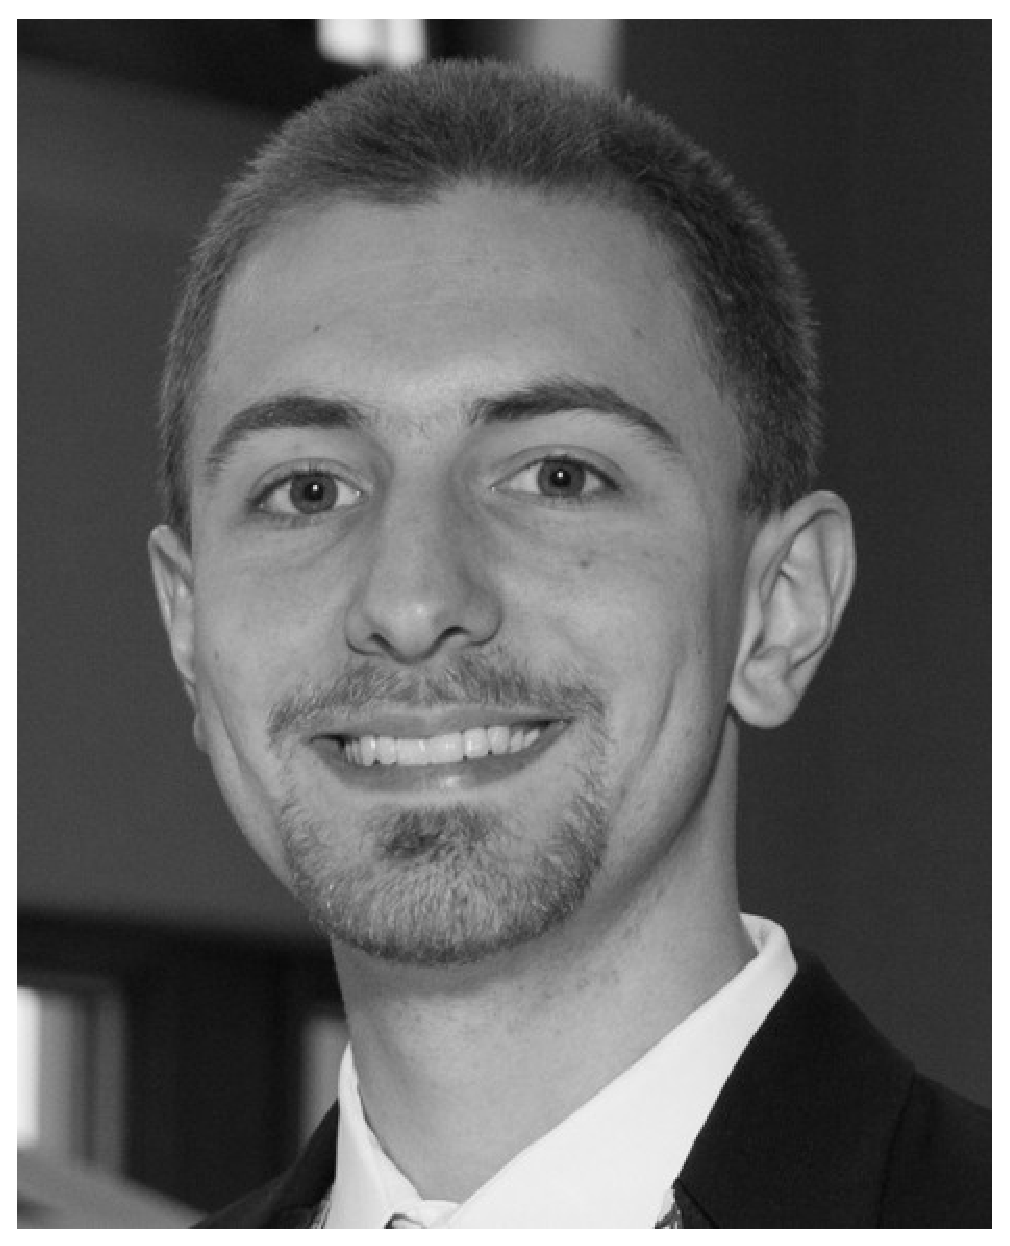
\includegraphics[width=1in,height=1.25in,clip,keepaspectratio]{goldman_headshot}}]{Brian W. Goldman}
received the B. S. degree and M.S. degree in computer science from the
Missouri University of Science and Technology, Rolla, in 2010
and 2012 respectively.

He is currently a Ph.D. student with the Department of Computer Science
and Engineering at Michigan State University, East Lansing.  His current
research interests include evolutionary computation and genetic programming.

\end{IEEEbiography}

% if you will not have a photo at all:
\begin{IEEEbiography}[{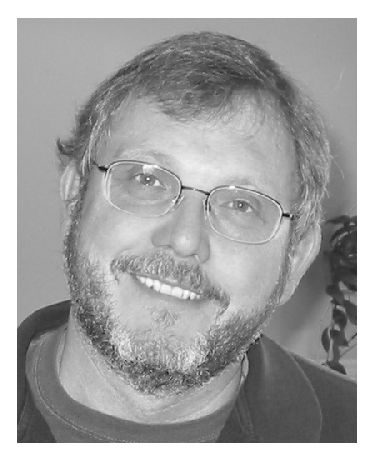
\includegraphics[width=1in,height=1.25in,clip,keepaspectratio]{headPunch}}]{William F. Punch}
Bill Punch received his Ph.D. from the Ohio State University and is currently an
Associate Professor at the Computer Science and Engineering Department of Michigan
State University. He is also the  director of the MSU High Performance Computing
Center. His research interests are evolutionary computation, high performance
computing and computing pedagogy. He co-directs the Genetic Algorithms Research
and Application Group (GARAGe) and is on the executive committee of the NSF STC,
BEACON, at MSU. His book with Rich Enbody titled "The Practice of Computing Using
Python" is now in its second edition.
\end{IEEEbiography}

% insert where needed to balance the two columns on the last page with
% biographies
%\newpage

% You can push biographies down or up by placing
% a \vfill before or after them. The appropriate
% use of \vfill depends on what kind of text is
% on the last page and whether or not the columns
% are being equalized.

%\vfill

% Can be used to pull up biographies so that the bottom of the last one
% is flush with the other column.
%\enlargethispage{-5in}



% that's all folks
\end{document}


